%  LaTeX support: latex@mdpi.com 
%  For support, please attach all files needed for compiling as well as the log file, and specify your operating system, LaTeX version, and LaTeX editor.

%=================================================================
\documentclass[quantumrep,article,submit,pdftex,moreauthors]{Definitions/mdpi}

%--------------------
% Class Options:
%--------------------
%----------
% journal
%----------
% Choose between the following MDPI journals:
% acoustics, actuators, addictions, admsci, adolescents, aerobiology, aerospace, agriculture, agriengineering, agrochemicals, agronomy, ai, air, algorithms, allergies, alloys, analytica, analytics, anatomia, animals, antibiotics, antibodies, antioxidants, applbiosci, appliedchem, appliedmath, applmech, applmicrobiol, applnano, applsci, aquacj, architecture, arm, arthropoda, arts, asc, asi, astronomy, atmosphere, atoms, audiolres, automation, axioms, bacteria, batteries, bdcc, behavsci, beverages, biochem, bioengineering, biologics, biology, biomass, biomechanics, biomed, biomedicines, biomedinformatics, biomimetics, biomolecules, biophysica, biosensors, biotech, birds, bloods, blsf, brainsci, breath, buildings, businesses, cancers, carbon, cardiogenetics, catalysts, cells, ceramics, challenges, chemengineering, chemistry, chemosensors, chemproc, children, chips, cimb, civileng, cleantechnol, climate, clinpract, clockssleep, cmd, coasts, coatings, colloids, colorants, commodities, compounds, computation, computers, condensedmatter, conservation, constrmater, cosmetics, covid, crops, cryptography, crystals, csmf, ctn, curroncol, cyber, dairy, data, ddc, dentistry, dermato, dermatopathology, designs, devices, diabetology, diagnostics, dietetics, digital, disabilities, diseases, diversity, dna, drones, dynamics, earth, ebj, ecologies, econometrics, economies, education, ejihpe, electricity, electrochem, electronicmat, electronics, encyclopedia, endocrines, energies, eng, engproc, entomology, entropy, environments, environsciproc, epidemiologia, epigenomes, est, fermentation, fibers, fintech, fire, fishes, fluids, foods, forecasting, forensicsci, forests, foundations, fractalfract, fuels, future, futureinternet, futurepharmacol, futurephys, futuretransp, galaxies, games, gases, gastroent, gastrointestdisord, gels, genealogy, genes, geographies, geohazards, geomatics, geosciences, geotechnics, geriatrics, grasses, gucdd, hazardousmatters, healthcare, hearts, hemato, hematolrep, heritage, higheredu, highthroughput, histories, horticulturae, hospitals, humanities, humans, hydrobiology, hydrogen, hydrology, hygiene, idr, ijerph, ijfs, ijgi, ijms, ijns, ijpb, ijtm, ijtpp, ime, immuno, informatics, information, infrastructures, inorganics, insects, instruments, inventions, iot, j, jal, jcdd, jcm, jcp, jcs, jcto, jdb, jeta, jfb, jfmk, jimaging, jintelligence, jlpea, jmmp, jmp, jmse, jne, jnt, jof, joitmc, jor, journalmedia, jox, jpm, jrfm, jsan, jtaer, jvd, jzbg, kidneydial, kinasesphosphatases, knowledge, land, languages, laws, life, liquids, literature, livers, logics, logistics, lubricants, lymphatics, machines, macromol, magnetism, magnetochemistry, make, marinedrugs, materials, materproc, mathematics, mca, measurements, medicina, medicines, medsci, membranes, merits, metabolites, metals, meteorology, methane, metrology, micro, microarrays, microbiolres, micromachines, microorganisms, microplastics, minerals, mining, modelling, molbank, molecules, mps, msf, mti, muscles, nanoenergyadv, nanomanufacturing,\gdef\@continuouspages{yes}} nanomaterials, ncrna, ndt, network, neuroglia, neurolint, neurosci, nitrogen, notspecified, %%nri, nursrep, nutraceuticals, nutrients, obesities, oceans, ohbm, onco, %oncopathology, optics, oral, organics, organoids, osteology, oxygen, parasites, parasitologia, particles, pathogens, pathophysiology, pediatrrep, pharmaceuticals, pharmaceutics, pharmacoepidemiology,\gdef\@ISSN{2813-0618}\gdef\@continuous pharmacy, philosophies, photochem, photonics, phycology, physchem, physics, physiologia, plants, plasma, platforms, pollutants, polymers, polysaccharides, poultry, powders, preprints, proceedings, processes, prosthesis, proteomes, psf, psych, psychiatryint, psychoactives, publications, quantumrep, quaternary, qubs, radiation, reactions, receptors, recycling, regeneration, religions, remotesensing, reports, reprodmed, resources, rheumato, risks, robotics, ruminants, safety, sci, scipharm, sclerosis, seeds, sensors, separations, sexes, signals, sinusitis, skins, smartcities, sna, societies, socsci, software, soilsystems, solar, solids, spectroscj, sports, standards, stats, std, stresses, surfaces, surgeries, suschem, sustainability, symmetry, synbio, systems, targets, taxonomy, technologies, telecom, test, textiles, thalassrep, thermo, tomography, tourismhosp, toxics, toxins, transplantology, transportation, traumacare, traumas, tropicalmed, universe, urbansci, uro, vaccines, vehicles, venereology, vetsci, vibration, virtualworlds, viruses, vision, waste, water, wem, wevj, wind, women, world, youth, zoonoticdis 
% For posting an early version of this manuscript as a preprint, you may use "preprints" as the journal. Changing "submit" to "accept" before posting will remove line numbers.

%---------
% article
%---------
% The default type of manuscript is "article", but can be replaced by: 
% abstract, addendum, article, book, bookreview, briefreport, casereport, comment, commentary, communication, conferenceproceedings, correction, conferencereport, entry, expressionofconcern, extendedabstract, datadescriptor, editorial, essay, erratum, hypothesis, interestingimage, obituary, opinion, projectreport, reply, retraction, review, perspective, protocol, shortnote, studyprotocol, systematicreview, supfile, technicalnote, viewpoint, guidelines, registeredreport, tutorial
% supfile = supplementary materials

%----------
% submit
%----------
% The class option "submit" will be changed to "accept" by the Editorial Office when the paper is accepted. This will only make changes to the frontpage (e.g., the logo of the journal will get visible), the headings, and the copyright information. Also, line numbering will be removed. Journal info and pagination for accepted papers will also be assigned by the Editorial Office.

%------------------
% moreauthors
%------------------
% If there is only one author the class option oneauthor should be used. Otherwise use the class option moreauthors.

%---------
% pdftex
%---------
% The option pdftex is for use with pdfLaTeX. Remove "pdftex" for (1) compiling with LaTeX & dvi2pdf (if eps figures are used) or for (2) compiling with XeLaTeX.

%=================================================================
% MDPI internal commands - do not modify
\firstpage{1} 
\makeatletter 
\setcounter{page}{\@firstpage}
\makeatother
\pubvolume{1}
\issuenum{1}
\articlenumber{0}
\pubyear{2023}
\copyrightyear{2023}
%\externaleditor{Academic Editor: Firstname Lastname}
\datereceived{ } 
\daterevised{ } % Comment out if no revised date
\dateaccepted{ } 
\datepublished{ } 
%\datecorrected{} % For corrected papers: "Corrected: XXX" date in the original paper.
%\dateretracted{} % For corrected papers: "Retracted: XXX" date in the original paper.
\hreflink{https://doi.org/} % If needed use \linebreak
%\doinum{}
%\pdfoutput=1 % Uncommented for upload to arXiv.org

%=================================================================
% Add packages and commands here. The following packages are loaded in our class file: fontenc, inputenc, calc, indentfirst, fancyhdr, graphicx, epstopdf, lastpage, ifthen, float, amsmath, amssymb, lineno, setspace, enumitem, mathpazo, booktabs, titlesec, etoolbox, tabto, xcolor, colortbl, soul, multirow, microtype, tikz, totcount, changepage, attrib, upgreek, array, tabularx, pbox, ragged2e, tocloft, marginnote, marginfix, enotez, amsthm, natbib, hyperref, cleveref, scrextend, url, geometry, newfloat, caption, draftwatermark, seqsplit
% cleveref: load \crefname definitions after \begin{document}

\usepackage{subfig}
%\usepackage{amsfonts}
\usepackage{xcolor}

\DeclareMathOperator{\tr}{tr}
\DeclareMathOperator{\Tr}{Tr}

%=================================================================
% Please use the following mathematics environments: Theorem, Lemma, Corollary, Proposition, Characterization, Property, Problem, Example, ExamplesandDefinitions, Hypothesis, Remark, Definition, Notation, Assumption
%% For proofs, please use the proof environment (the amsthm package is loaded by the MDPI class).

%=================================================================
% Full title of the paper (Capitalized)
\Title{Tomographic Universality of the Discrete Wigner Function}

% MDPI internal command: Title for citation in the left column
\TitleCitation{Tomographic Universality of the Discrete Wigner Function}

% Author Orchid ID: enter ID or remove command
\newcommand{\orcidauthorA}{0000-0002-6671-0262} % Add \orcidA{} behind the author's name
\newcommand{\orcidauthorB}{0009-0009-9564-9542} % Add \orcidB{} behind the author's name
\newcommand{\orcidauthorC}{0000-0002-5210-0981} % Add \orcidC{} behind the author's name
\newcommand{\orcidauthorD}{0000-0001-8493-721X} % Add \orcidD{} behind the author's name

% Authors, for the paper (add full first names)
\Author{
  Isabel Sainz $^{1,\dagger}$\orcidA{},
  Ernesto Camacho $^{2,\dagger}$\orcidB{},
  Andrés García $^{2,\dagger}$\orcidC{}
  and Andrei B. Klimov $^{1,*,\dagger}$\orcidD{}.
}

%\longauthorlist{yes}

% MDPI internal command: Authors, for metadata in PDF
\AuthorNames{Isabel Sainz, Ernesto Camacho, Andrés García and Andrei B. Klimov}

% MDPI internal command: Authors, for citation in the left column
\AuthorCitation{Sainz, I.; Camacho, E.; García, A.; Klimov, A.B.;}
% If this is a Chicago style journal: Lastname, Firstname, Firstname Lastname, and Firstname Lastname.

% Affiliations / Addresses (Add [1] after \address if there is only one affiliation.)
\address{%
  $^{1}$ \quad Departamento de Física, Universidad de Guadalajara, Revolución
    1500, 44420, Guadalajara, Jal., México\\
  $^{2}$ \quad Departamento de Matemáticas, Universidad de Guadalajara,
    Revolución 1500, 44420, Guadalajara, Jal., México\\
}

% Contact information of the corresponding author
\corres{Correspondence: andrei.klimov@academicos.udg.mx.}

% Current address and/or shared authorship
\firstnote{These authors contributed equally to this work.}
%\secondnote{Current address: Affiliation 3.} 
% The commands \thirdnote{} till \eighthnote{} are available for further notes

%\simplesumm{} % Simple summary

%\conference{} % An extended version of a conference paper

% Abstract (Do not insert blank lines, i.e. \\) 
\abstract{
  We observe that the Discrete Wigner function (DWF) for $n$-partite systems
  with odd local dimensions are tomographically universal, as reflected in a
  delta-function form of the DWF for any stabilizer. However, in the $n$-qubit
  case this property does not hold due to the non-factorization of the mapping
  kernel, whose explicit form depends on a particular partition of the discrete
  phase-space. Nonetheless, it turns out that the DWF for some specific
  stabilizers, not included in the set used for the construction of the Wigner
  map, takes on the form of a delta-function. This implies that the possibility
  of classical simulations of Pauli measurements in a given stabilizer state for
  qubit systems is closely tied to the experimental setup.
}

% Keywords
\keyword{
  discrete Wigner function; quantum tomography; stabilizer formalism; Mutually
  Unbiased Bases.
} 

% The fields PACS, MSC, and JEL may be left empty or commented out if not applicable
%\PACS{J0101}
%\MSC{}
%\JEL{}

%%%%%%%%%%%%%%%%%%%%%%%%%%%%%%%%%%%%%%%%%%
\begin{document}

%%%%%%%%%%%%%%%%%%%%%%%%%%%%%%%%%%%%%%%%%%
\section{Introduction}

The concept of quasidistribution functions, which emerged as a means to
incorporate quantum corrections into statistical mechanics within two distinct
contexts \cite{wigner,bloch}, has been successfully used to reformulate quantum
mechanics in position and momentum (plane) phase space \cite{groenewold,moyal}.
Subsequently, these concepts were generalized to more sophisticated geometries.
In the framework of the phase-space approach, operators suitable for a given
quantum system are represented as real functions obtained from an invertible and
covariant linear map $\hat{w}(\Omega)$,

\begin{equation*}
  \hat{f}\Leftrightarrow W_{f}(\Omega)
  = \Tr\left(\hat{f}\hat{w}(\Omega)\right),
\end{equation*}

where $\Omega$ is a point in the corresponding phase-space $\mathcal{M}$.

The most natural and widely used representation
\cite{qoptics,electron1,electron2} commonly referred to as the Wigner
correspondence \cite{wigner} is self-dual. This self-duality allows for the
treatment of both states and observables in the same manner, making it
particularly useful for studying the quantum-classical correspondence
\cite{berry}. However, the main drawback of the Wigner map lies in its
representation of some states in the form of negative (quasi)-distributions. In
fact, it's noteworthy that non-negative Wigner functions (WF) correspond only to
the so-called Gaussian states, thereby restricting the type of
positivity-preserving operations to Gaussian ones.

A discrete analogue of the Wigner map, which is applicable for describing a
finite number of particles with a local dimension that is a prime number,
was introduced significantly later \cite{spin1, spin2,wootters1,gibbons}.
This discrete analog has recently found remarkable applications in the
analysis of classicality and the (classical) simulability of $n$-partite
quantum systems \cite{gottKnill, galvao, cormick, gross,WignerNegResource,
Raus17, UniqueWF, cohomo}. In this context, the discrete phase-space (DPS)
$\mathcal{M}$ takes the form of a $p^{n}\times p^{n}$ grid, constituting an
affine plane \cite{Saniga2004}. By labeling it with elements from the Galois
field $\mathbb{F}_{p^{n}}$ , this DPS inherits the same geometric properties as
the ordinary plane, e.g., parallel lines (not necessarily straight) do not
intersect, etc.

The construction of discrete quasidistributions is closely tied to the concept
of Mutually Unbiased Bases (MUBs) \cite{ivanovic,mubs1,mubs2}, which are
eigenstates of disjoint sets of $p^{n}$ commuting monomials (stabilizers) formed
by products of the generalized Pauli operators. In power-of-prime dimensions one
can always arrange the operational basis formed by $p^{2n}-1$ monomials
(excluding the identity operator) into $p^{n}+1$ disjoint stabilizers
~\cite{Bandyopadhyay2002}. \textbf{\color{teal}In addition, it is possible to
associate lines in the DPS with projectors onto elements of a certain
(stabilizer) basis in a way that parallel lines correspond to different
components of the same basis, while (single) intersecting lines are related to
states belonging to the mutually unbiased bases} \cite{wootters1}. It is
noteworthy that in the prime-dimensional case only straight lines can be related
to MUBs.  However, in power-of-prime dimensions such an association exists with
more complex geometrical structures, the so-called commutative curves
\cite{GS2,JPA09}. This leads to a fundamental property of the discrete Wigner
function: the tomographic condition. This condition means that summing the
Wigner function over a line results in the probability that the system is in the
state associated with that particular line \cite{wootters1, gibbons}.

The mapping kernel from the Hilbert space into the DPS can be recast as a sum of
projectors onto elements of an appropriate complete set of MUBs.  However, there
are several inequivalent ways to form $p^{n}+1$ disjoint commuting sets, which
correspond to different partitions of the DPS into non-intersecting curves. Such
sets can be roughly characterized by their factorization properties and both
unitary equivalent and (globally) unitary inequivalent sets of stabilizers can
be found. Consequently, the form of the discrete self-dual maps fundamentally
depends on the chosen complete set of stabilizers \cite{Bjork2007}. For each
state of the MUBs used in the construction of the mapping kernel, the Wigner
function is represented as a delta-function. The later is equivalent to the
tomographic condition \cite{gibbons,galvao,cormick,DFW11,DFW12}.

On the other hand, it's known that the Wigner map for odd-prime local dimensions
exhibits a property akin to the continuous position-momentum Wigner function:
only stabilizer states correspond to non-negative Wigner functions \cite{gross}.
This characteristic arises from the factorization of the self-dual mapping
kernel for any partition of the DPS and results in tomographic universality of
the DWFs, which acquire a delta-function form for any stabilizer state of any
partition. It enables the use of the DWF as an indicator of quantumness,
allowing the classification of quantum states based on their suitability for
quantum computation speedup and estimation of the cost of classically simulating
quantum circuits \cite{Raus17,UniqueWF, cohomo, contextMagic, WignerContext}.

However, this property breaks down in the case of qubit systems \cite{UniqueWF,
cohomo,contextMagic}. The main reason for the loss of tomographic universality
in $n$-qubit systems is the inequivalence among Wigner maps based on different
sets of stabilizers \cite{Bjork2007}, \cite{qip17}. This leads to the following
question: Is it possible for the DWF of an element of a stabilizer basis to take
on the form of a delta-function if that basis is not used for the construction
of the Wigner map? In other words, are there states, aside from the elements of
the MUBs fixing the map, that satisfy the tomographic condition?

In this paper, we show that in the $n$-qubit case, when a partition of the
discrete phase-space into a complete fixed set of stabilizers is given, it is
possible to identify stabilizer states whose Wigner functions take on the form
of delta functions along commutative curves belonging to other partitions. We
analyze explicit results for the three-qubit case and discuss the implications
of this observed property of $n$-qubit DWFs.

\textbf{\color{teal}The structure of this paper is as follows: In Sec. 2 we
  recall the basic properties of $n$-qudit operations in the Hilbert space, in
  particular: the construction of abelian displacement operators and the
  relation to different types of MUBs. In Sec. 3 we discuss geometric structures
  related to MUBs in the discrete phase-space and which are employed for the
  construction of the Wigner map. In Sec. 4 we focus on the tomographic
  universality of $n$-qudit Wigner functions for odd local dimensions and on
  identifying the stabilizer states with non-negative delta-like Wigner
  functions in the $n$-qubit case.}

%%%%%%%%%%%%%%%%%%%%%%%%%%%%%%%%%%%%%%%%%%

\section{The generalized Pauli group and displacement operators}

Let us consider a system of $n$ qudits, each with a \textit{local} dimension
that is a prime number $p$. It is convenient to relabel vectors of an
orthonormal basis $|k_{1}, \ldots, k_{n}\rangle$, $k_{i}\in \mathbb{Z}_{p}$ in
the corresponding Hilbert space $\mathcal{H}_{p^{n}}=\mathcal{H}_{p}^{\otimes
n}$ by elements of a finite field, $|\kappa \rangle$, $\kappa \in
\mathbb{F}_{p^{n}}$ according to

\begin{equation}
  |k_{1}, \ldots, k_{n}\rangle
  \Leftrightarrow |\kappa\rangle, \quad \langle\kappa^{\prime}|\kappa\rangle
  = \delta_{\kappa^{\prime},\kappa}, \quad \kappa =
  \sum_{i=1}^{n} k_{i} \, \theta_{i} \in \mathbb{F}_{p^{n}},
  \label{basis}
\end{equation}

where $\{\theta_{1},\ldots,\theta_{n}\}$ is an abstract basis in the field
$\mathbb{F}_{p^{n}}$, considered as a linear space; the components $k_{i}$,
$i=1,..,n$ are obtained through the trace operation with a dual basis, $\{
\tilde{\theta}_{1},\ldots ,\tilde{\theta}_{n}\}$ [i.e., $\tr(\theta _{i}\,
\tilde{\theta}_{j})=\delta _{ij}$], here $\tr(\alpha) = \alpha
+\alpha^{2}+\ldots + \alpha ^{p^{n-1}}$, for $\alpha \in \mathbb{F}_{p^{n}}$
\cite{FF}.

In even dimensions there always exists a self-dual basis, i.e. a basis such that
$\tr(\theta_{i}\,\theta_{j})=\delta_{ij}$, whereas in odd dimensions there are
\textit{almost} self-dual bases, such that
$\tr(\theta_{i}\,\theta_{j})=q_{j}\delta_{ij}$, where $q_{j}$ is equal to $1$
with one possible exception, e.g. $q_{j} = (q-1)\delta_{jn}+1$ for some $q \in
\mathbb{Z}_p$.

The generators of the Pauli group $\mathcal{P}_{n}$ can be expressed as,

\begin{eqnarray}
  \hat{Z}_{\alpha }
  &=& \sum_{\kappa } \chi\left( \alpha \kappa \right)
  |\kappa \rangle \langle \kappa|,
  \qquad \hat{X}_{\beta }
  = \sum_{\kappa} |\kappa + \beta \rangle \langle \kappa|,
  \label{XZ} \\
  \hat{Z}_{\alpha }^{\dagger}
  &=& \hat{Z}_{-\alpha}, \quad \hat{X}_{\beta }^{\dagger}
  = \hat{X}_{-\beta}, \quad \hat{Z}_{\alpha}^{p}
  = \hat{X}_{\beta}^{p} = \hat{I},
\end{eqnarray}

where

\begin{equation*}
  \chi \left( \alpha \right)
  = \omega^{tr\left( \alpha \right)},
  \quad \omega = e^{2\pi i / p},
\end{equation*}

are additive characters of the finite field,

\begin{equation*}
  \chi\left( \alpha +\beta \right)
  = \chi\left( \alpha \right) \chi\left( \beta \right),
  \qquad \sum_{\kappa }\chi \left( \kappa \alpha \right)
  = p^{n}\delta_{\alpha, 0}.
\end{equation*}

The operators (\ref{XZ}) satisfy the discrete counterpart of the Weyl form of
the commutation relations,

\begin{equation}
  Z_{\alpha}X_{\beta }
  = \chi \left( \alpha \beta \right) \, X_{\beta }Z_{\alpha} \,.
  \label{commutation_relation}
\end{equation}

In an almost self-dual basis the character of a product of field elements is
factorized:

\begin{equation}
  \chi\left( \alpha \beta \right)
  %= \Pi_{j=1}^{n} \omega{\left( \alpha_{j}\beta_{j}q_{j}\right)},
  = \Pi_{j=1}^{n} \omega^{\alpha_{j}\beta_{j}q_{j}},
  \label{chi fact}
\end{equation}

where $a_{i} = \tr(\alpha \tilde{\theta}_{i})$ and $b_{i} = \tr(\beta
\tilde{\theta }_{i})$. This implies a factorization of $\hat{Z}_{\alpha}$ and
$\hat{X}_{\beta }$ into a product of cyclic operators
\cite{Schwinger1,Schwinger2},

\begin{equation}
  \hat{Z}
  = \sum_{n=0}^{p-1} \omega^{n} |n\rangle \langle n|, \quad \hat{X}
  = \sum_{n=0}^{p-1} |n+1\rangle \langle n|,
  \quad \hat{X}^{p} = \hat{Z}^{p} = \hat{I},
  \quad \hat{Z}\hat{X} = \omega \hat{X}\hat{Z}.
\end{equation}

according to

\begin{equation}
  \hat{Z}_{\alpha }
  = \otimes \Pi_{j}\hat{Z}^{q_{j}a_{j}},
  \qquad \hat{X}_{\beta} = \otimes \Pi _{j}\hat{X}^{b_{j}}.
  \label{ZXq}
\end{equation}

The monomials $\{\hat{Z}_{\alpha }\hat{X}_{\beta }$, $\alpha ,\beta \in
\mathbb{F}_{p^{n}}\}$ form an operational basis in $Op[\mathcal{H}_{p^{N}}]$ and
can be arranged in commuting sets of unitary displacement operators
$\hat{D}(\alpha,\beta)$ obtained by Clifford transformations
$\hat{U}_{\alpha,\beta}$ of the set $\{\hat{Z}_{\tau}$, $\tau \in
\mathbb{F}_{p^{n}}\}$:

\begin{equation}
  \hat{D} \left( \alpha (\tau ),\beta (\tau )\right)
  = \Phi_{\alpha,\beta} \left( \tau \right)
  \hat{Z}_{\alpha (\tau)}\hat{X}_{\beta(\tau)}
  = \hat{U}_{\alpha,\beta}\hat{Z}_{\tau}\hat{U}_{\alpha,\beta }^{\dagger}
  = \hat{D}^{\dagger }\left(\alpha (-\tau),\beta (-\tau )\right),
  \label{D}
\end{equation}

where $\Phi_{\alpha ,\beta }\left( \tau \right) \Phi_{\alpha ,\beta }^{\ast
}\left( \tau \right) = 1$ is a phase factor. The operators (\ref{D}) from each
commuting set $\lambda =\{\alpha ,\beta\}$ form an abelian group,

\begin{equation}
  \hat{D}\left( \alpha_{\lambda}(\tau),\beta_{\lambda }(\tau) \right)
  \hat{D}\left(
    \alpha_{\lambda}(\tau^{\prime }),\beta_{\lambda }(\tau^{\prime })
  \right)
  = \hat{D}\left(
    \alpha_{\lambda}(\tau + \tau^{\prime}),
    \beta_{\lambda}(\tau + \tau^{\prime})
  \right),
  \label{DD}
\end{equation}

as a consequence of the relation $\hat{Z}_{\tau }\hat{Z}_{\tau ^{\prime}} =
\hat{Z}_{\tau +\tau^{\prime}}$. This implies that the phases $\Phi_{\alpha,\beta
}\left( \tau \right) $, where $(\alpha ,\beta )\in \lambda$, $\Phi_{\alpha
,\beta }\left( 0\right) = 1$ satisfy the equation,

\begin{equation}
  \Phi_{\alpha,\beta}\left( \tau \right)
  \Phi_{\alpha,\beta }\left(\tau^{\prime}\right)
  = \Phi_{\alpha,\beta }\left( \tau +\tau^{\prime}\right)
  \chi\left(\alpha_{\lambda}(\tau^{\prime})\beta_{\lambda}(\tau)\right)
  = \Phi_{\alpha,\beta}\left(\tau + \tau^{\prime}\right)
  \chi\left(\alpha_{\lambda}(\tau)\beta_{\lambda}(\tau^{\prime })\right),
  \label{Phi}
\end{equation}

leading to the following condition for the labels of elements of $\lambda$:

\begin{equation}
  \tr\left(\alpha_{\lambda}(\tau^{\prime })\beta_{\lambda }(\tau)\right)
  = \tr\left(\alpha_{\lambda}(\tau)\beta_{\lambda }(\tau^{\prime })\right),
  \quad \tau,\tau^{\prime} \in \mathbb{F}_{p^{n}}.
  \label{CC}
\end{equation}

The eigenstates $|\psi_\kappa^\lambda\rangle$ of each commuting set
$\{\hat{D}\left(\alpha_{\lambda}(\tau),\beta_{\lambda}(\tau)\right) \equiv
\hat{D}^{\lambda}(\tau)$, $\tau \in \mathbb{F}_{p^{n}}\}$,

\begin{equation}
  \hat{D}^{\lambda}(\tau) |\psi_{\kappa}^{\lambda}\rangle
  = \chi(\kappa \tau) |\psi_{\kappa}^{\lambda }\rangle,
  \quad \kappa \in \mathbb{F}_{p^{n}},
  \label{states}
\end{equation}

form an orthonormal basis in $\mathcal{H}_{p^{n}}$. The disjoint sets of
displacement operators satisfy the relation,

\begin{equation*}
  \Tr\left(
    \hat{D}^{\lambda^{\prime}}(\tau^{\prime})\hat{D}^{\lambda\dagger}(\tau)
  \right)
  = p^{n} \delta_{\lambda,\lambda^{\prime}} \delta_{\tau,\tau^{\prime }}
  + p^{n}(1 - \delta_{\lambda,\lambda^{\prime}}) \delta_{\tau,0}
  \delta_{\tau^{\prime},0},
\end{equation*}

and so the corresponding bases (\ref{states}) are mutually unbiased,

\begin{equation}
  |\langle\psi_{\kappa^{\prime}}^{\lambda^{\prime}}
  |\psi_{\kappa}^{\lambda}\rangle|^{2}
  = \delta_{\lambda,\lambda^{\prime}} \delta_{\kappa,\kappa^{\prime}}
  + p^{-n} (1-\delta_{\lambda,\lambda^{\prime}}).
  \label{UB}
\end{equation}

Commuting sets of displacement operators $\{\hat{D}^{\lambda }(\tau ),\tau \in
\mathbb{F}_{p^{n}}\}$, containing $p^{n}-1$ monomials (excluding the identity
operator), are usually called stabilizers and the respective eigenstates are the
stabilizer states. The entire set of $p^{2n}-1$ monomials can be partitioned
into $p^{n}+1$ disjoint stabilizers in several locally inequivalent forms, i.e.,
they cannot be reduced to each other through local transformations. This is
related to a possibility of constructing stabilizers with different
factorization structures \cite{factor1,factor2}, which are related to the
commutation condition between blocks of single-qudit operators (\ref{ZXq})
constituting commutative sets ($\lambda$) of direct products of $n$
generalized Pauli operators. Each monomial (up to a phase),

\begin{equation*}
  \hat{Z}_{\alpha(\tau)}\hat{X}_{\beta(\tau)}
  = \otimes \Pi_{j} \left(
    \hat{Z}^{q_{j}a_{j}(\tau)}\hat{X}^{b_{j}(\tau)}
  \right),
  \quad \tau \in \mathbb{F}_{p^{n}},
  \quad \left(\alpha(\tau),\beta(\tau)\right) \in \lambda,
\end{equation*}

can be divided into two parts, so that the first part contains $k$ operators,
corresponding to the $(j_{1},\ldots ,j_{k})$ qudits and the second part contains
the $n-k$ operators of the rest of the qudits. The stabilizer is factorized into
at least two subsets if the products of Pauli operators from the first blocks of
the all monomials commute between each other (the operators from all the second
blocks satisfy the same condition).  Some mutually commuting sub-blocks may
exist inside the first or second blocks, etc. Thus, one can represent any
stabilizer $\lambda $ in the following form

\begin{equation}
  \lambda = \{m_{1}, m_{2}, \ldots, m_{n}\},
  \label{curve_part}
\end{equation}

where $0<m_{1}\leq m_{2}\leq \ldots \leq m_{N}$ and $\sum_{j}m_{j}=n$ is the
number of qudits in the $j-$th block that cannot be factorized into commuting
sub-blocks anymore. The partition $\lambda =\underbrace{\{1,1,\ldots ,1\}}_{n}$
corresponds to a completely factorized stabilizer and $\lambda $ $=\{n\}$ to a
completely non-factorized one. It is worth noting that different partitions may
have the same factorization structure.

The simplest complete set of stabilizers is labelled by linear functions:

\begin{equation}
  \alpha = \tau, \quad \beta = \mu \tau, \quad \mu \in \mathbb{F}_{p^{n}};
  \quad \alpha = 0,
  \label{rays}
\end{equation}

where the commuting sets $\left(\alpha = \tau, \beta = \tau \right)$,
$\left(\alpha = 0\right)$, $\left(\beta = 0\right)$ are always completely
factorized.  However, the factorization structure for the other values of $\mu$
depends on the number of qudits and the local dimensions.

More sophisticated dependences of pairs
$\left(\alpha_{\lambda}(\tau),\beta_{\lambda }(\tau)\right)$ over the parameter
$\tau$ have the form \cite{GS2,JPA09},

\begin{equation}
  \alpha_{\lambda }(\tau)
  = \sum_{m=0}^{n-1} \alpha_{m}^{\lambda } \,
  \tau^{p^{m}}, \qquad \beta_{\lambda}(\kappa)
  = \sum_{m=0}^{n-1}\beta_{m}^{\lambda} \, \tau^{p^{m}},
  \label{curve1}
\end{equation}

where the coefficients $\alpha_{m}$, $\beta _{m}$ $\in \mathbb{F}_{p^{n}}$
should satisfy conditions derived from (\ref{CC}), as, for instance,

\begin{equation*}
  \sum_{m \neq k} \tr(\alpha_{m}\beta _{k}) = 0, \quad k = 0,...,n.
\end{equation*}

It's worth noting that the displacement operators belonging to a given
stabilizer $\lambda $ can be expanded into the projectors of the corresponding
basis vectors $\{|\psi _{\kappa }^{\lambda }\rangle ,\kappa \in
\mathbb{F}_{p^{n}}\}$,

\begin{equation}
  \hat{D}^{\lambda }(\tau )
  = p^{-n} \sum_{\kappa }\chi (\kappa \tau )
  |\psi _{\kappa }^{\lambda }\rangle \langle \psi _{\kappa }^{\lambda }|.
  \label{Dexp}
\end{equation}

The above equation allows us to represent any state in terms of the
probabilities $p_{\kappa }^{(\lambda )} = \langle \psi_{\kappa
}^{\lambda}|\hat{\rho}|\psi _{\kappa }^{\lambda }\rangle $ of projections onto
elements of MUBs, i.e. tomographically reconstruct the state
\cite{gibbons,galvao,cormick,ivanovic,DFW11,DFW12,Durt2006}:

\begin{equation}
  \hat{\rho}
  = \sum_{\lambda }\sum_{\kappa }
  p_{\kappa}^{(\lambda)} |\psi_{\kappa }^{\lambda }\rangle
  \langle \psi _{\kappa }^{\lambda }| - \hat{I}
  = \sum_{\lambda }\sum_{\kappa }\left( p_{\kappa }^{(\lambda)} -
  \frac{1}{p^{n}+1}\right) |\psi _{\kappa }^{\lambda }\rangle \langle
  \psi_{\kappa }^{\lambda }|.
  \label{tom r}
\end{equation}

%%%%%%%%%%%%%%%%%%%%%%%%%%%%%%%%%%%%%%%%%%

\section{Phase space construction and the Wigner map}

The discrete phase-space (DPS) \cite{gibbons,galvao,cormick,DFW11,DFW12} is a
$p^{n}\times p^{n}$ grid, where the points $(\alpha ,\beta )$, $\alpha,\beta \in
\mathbb{F}_{p^{n}}$ label elements of monomials $\hat{Z}_{\alpha
}\hat{X}_{\beta}$. This DPS is endowed with a finite geometry
\cite{gibbons,galvao,cormick,DFW11,DFW12,FF}, and admits a set of discrete
symplectic transformations \cite{DFW2-1,DFW2-2,DFW2-3,DFW2-4,klimov06}.
Similarly to the continuous case, the axes of the DPS are associated with the
observables $\hat{Z}_{\alpha}$ and $\hat{X}_{\beta}$.

A separation of $Op[\mathcal{H}_{p^{n}}]$ into disjoint stabilizers corresponds
to a partition of the DPS into non-intersecting (except at the origin),
non-degenerate (containing $p^{n}$ different points including the origin)
\textit{commutative} curves $\{\Gamma =\left( \alpha (\tau ),\beta
(\tau)\right), \; \tau \in \mathbb{F}_{p^{n}}\}$ \cite{GS2,JPA09}.
\textbf{\color{teal} In other words, the points of every commutative curve
$\Gamma$ label a set of mutually commutative monomials,}

\begin{equation}
  \{\hat{Z}_{\alpha (\tau )}\hat{X}_{\beta (\tau )}, \;
  [\hat{Z}_{\alpha(\tau)} \hat{X}_{\beta (\tau )},
  \hat{Z}_{\alpha (\tau ^{\prime })}\hat{X}_{\beta(\tau^{\prime })}]
  = 0, \; \left( \alpha (\tau ),\beta (\tau )\right) \in \Gamma \},
\end{equation}

\textbf{\color{teal} such that the condition (\ref{CC}) is satisfied. There
exist $p^{n}+1$ commutative curves $\Gamma^{\lambda }$ in every DPS partition,
so that the index $\lambda$, labelling curves within a given partition, takes
$p^{n}+1$ distinct values.} In addition, there are $p^{n}-1$ parallel curves
$\{\Gamma _{\kappa }^{\lambda}$, $\kappa \in \mathbb{F}_{p^{n}}\}$ for each
curve passing through the origin.  The whole bundle of $p^{n}$ parallel curves
(called a striation) covers the DPS, \textbf{\color{teal} and at every
phase-space point $p^{n}+1$ curves (i.e.  one curve from each striation)
intersect. It is worth stressing that only the monomials, labelled by the points
of the curves crossing the origin, commute among each other.}

The set of rays (\ref{rays}) is the simplest example of such a partition, where
the sets of parallel lines are explicitly defined as,

\begin{eqnarray}
  \beta
  &=& \mu \alpha + \kappa, \quad \mu, \kappa \in \mathbb{F}_{p^{n}}
  \quad \text{($p^{n}$ sets)}
  \label{rays0} \\
  \alpha
  &=& \kappa, \quad \kappa \in \mathbb{F}_{p^{n}},
  \quad \text{ (a single set).}
  \notag
\end{eqnarray}

Another way to establish a connection between the discrete geometry with the
algebraic structures is to link the commutative curves with the eigenstates
(\ref{states}) of the corresponding stabilizers. This approach associates each
basis $\{|\psi _{\kappa }^{\lambda }\rangle $, $\kappa \in F_{p^{n}}\}$ with a
striation of curves $\{\Gamma_{\kappa }^{\lambda } = \left( \alpha_{\lambda
}(\tau ,\kappa ),\beta_{\lambda }(\tau ,\kappa )\right) ,\,\tau \in
\mathbb{F}_{p^{n}}\}$, and the bases corresponding to different striations are
mutually unbiased. In the conventional association, the curves that include the
origin are put in correspondence with the states $|\psi_{\kappa = 0}^{\lambda
}\rangle $ with unit eigenvalues (later called the unit stabilizer states). Such
curves $\Gamma_{\kappa =0}^{\lambda }\equiv \Gamma^{\lambda }$, have the form
(\ref{curve1}) and will be called unit commutative curves. 

Both $n$-qudit states and observables can be represented in the form of
distributions in the DPS through a one-to-one map
\cite{gross,DFW2-1,DFW2-2,DFW2-3,DFW2-4},

\begin{align}
  W_{f}\left( \alpha ,\beta \right)
  &= \Tr \left[ \hat{f}\hat{w}\left(\alpha ,\beta \right) \right],
  \label{map} \\
  \hat{f}
  &= p^{-n}\sum_{\alpha, \beta } W_{f}(\alpha,\beta) \hat{w}(\alpha,\beta),
\end{align}

where the Hermitian mapping kernel $\hat{w}\left( \alpha ,\beta \right) =
\hat{w}^{\dagger }(\alpha ,\beta )$ is covariant under action of the discrete
displacements (\ref{D}), and is defined as

\begin{eqnarray}
  \hat{w}\left( \alpha ,\beta \right)  &=&\hat{D}\left( \alpha ,\beta \right) 
  \hat{w}\left( 0,0\right) \hat{D}^{\dagger }\left( \alpha ,\beta \right) ,
  \label{Ds} \\
  \hat{w}\left( 0,0\right)  &=&\sum_{\gamma ,\delta }\hat{D}(\gamma ,\delta ),
  \label{Dw0}
\end{eqnarray}

\textbf{\color{teal} so that}

\begin{equation}
  \color{teal}
  \boldmath
  \hat{w} \left( \alpha, \beta \right)
  = p^{-n} \sum_{\gamma, \delta}
  \chi(\gamma \beta -\delta \alpha) \hat{D}(\gamma, \delta).
  \label{wabD}
\end{equation}

The kernel (\ref{Ds}) is normalized according to,

\begin{equation}
  \sum_{\alpha,\beta}\hat{w}\left(\alpha,\beta\right)
  = p^{n}\hat{I},
\end{equation}

and satisfies the overlap relation,

\begin{equation}
  \Tr\left(\hat{w}(\alpha,\beta)\hat{w}(\alpha^{\prime},\beta^{\prime})\right)
  = p^{n} \delta_{\alpha \alpha^{\prime}} \delta_{\beta\beta^{\prime}}.
\end{equation}

It is convenient to recast Eq. (\ref{Dw0}) as a sum of stabilizers corresponding
to a given phase-space partition,

\begin{equation}
  \hat{w}\left(0,0\right)
  = p^{-n} \sum_{\lambda} \sum_{\tau} \hat{D}^{\lambda}(\tau)-\hat{I},
  \label{Dw00}
\end{equation}

or, equivalently, as a plane superposition of projectors onto the elements of
MUBs:

\begin{equation}
  \hat{w}\left( 0,0\right)
  = \sum_{\lambda } |\psi _{0}^{\lambda }\rangle
  \langle \psi _{0}^{\lambda }| - \hat{I},
  \label{w0}
\end{equation}

where the index $\lambda$, labels the stabilizers/projectors (\ref{states})
within this partition. Geometrically, Eqs. (\ref{Dw00}) and (\ref{w0}) represent
a summation along the curves that pass through the origin, i.e. of the form
(\ref{curve1}). In other words, each point $(\alpha, \beta)$ of the DPS is
assigned a specific phase $\Phi_{\alpha, \beta}\left( \tau \right)$ according
to the unit commutative curve $\Gamma^{\lambda}$ that passes through that point
and corresponding to the displacement operator
$D\left(\alpha_{\lambda}(\tau),\beta_{\lambda}(\tau)\right)$.
\textbf{\color{teal} In Figure~\ref{fig1} we plot all of the unit commutative
  curves $\{\Gamma^{\lambda}\}$ and the distribution of the corresponding phases
  $\{\Phi_{\alpha,\beta},(\alpha,\beta) \in \Gamma^{\lambda}\}$ along each
curve, in the case of three qubits for two different partitions.}

\begin{figure}[ht]
  \color{teal}
  \centering
  \subfloat[\centering]{{
    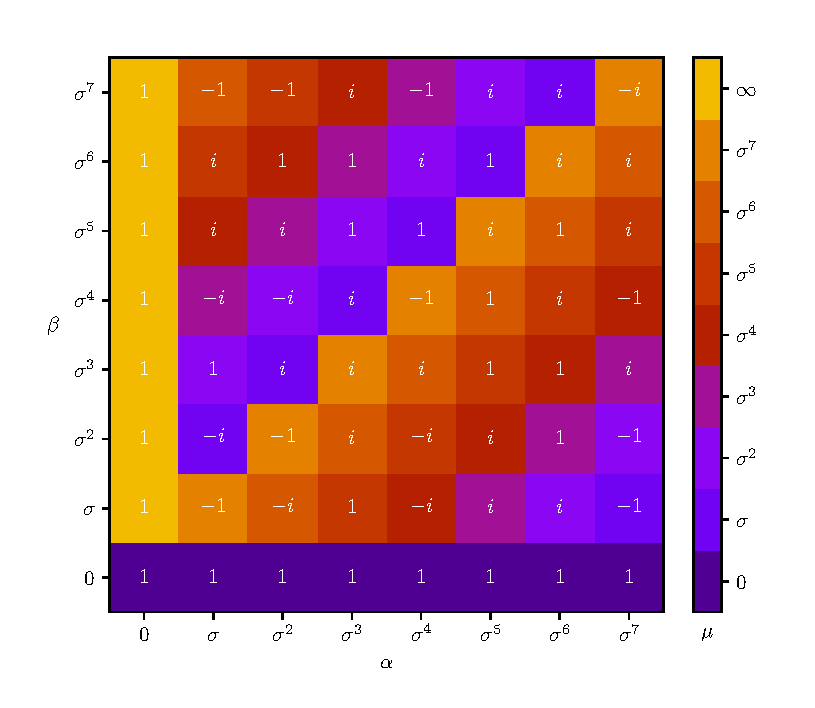
\includegraphics[width=6.9cm]{DPS_rays_heat.eps}
  }}
  \subfloat[\centering]{{
    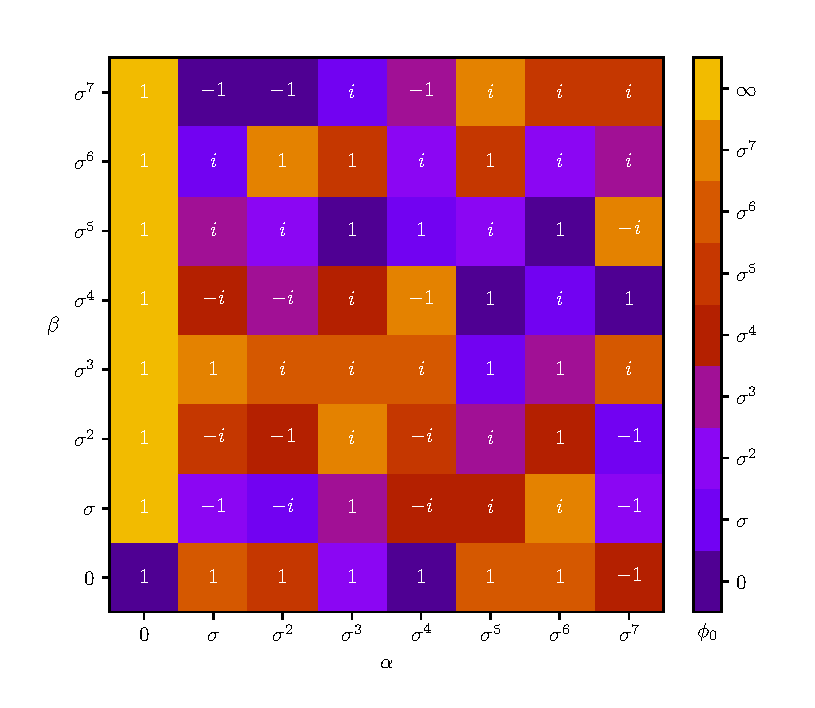
\includegraphics[width=6.9cm]{DPS_curve_heat.eps}
  }}
  \caption{\textbf{
    \color{teal}
    Unit commutative curves along with the distribution of the respective phases
    (\ref{D}) satisfying the condition (\ref{Phi}) for the partitions: (a),
    $(3,0,6)$ described by the rays $\beta = \mu \alpha$, $\alpha = 0$, $\mu \in
    \mathbb F_{2^{3}}$; (b), $(1,6,2)$ described by the curves $\beta = \mu
    \alpha + \alpha^2 + \alpha^{4}$, $\mu \in \mathbb F_{2^{3}}$.
  }}
  \label{fig1}
\end{figure}

By shifting $\hat{w}\left(0,0\right)$ through the action of the displacement
operators (\ref{Ds}) to an arbitrary point $(\alpha,\beta )$ one obtains

\begin{equation}
  \hat{w}(\alpha, \beta)
  = \sum_{\lambda(\alpha,\beta),\kappa(\alpha,\beta)}
  |\psi _{\kappa }^{\lambda }\rangle \langle \psi _{\kappa }^{\lambda }|
  - \hat{I},
  \label{wab}
\end{equation}

where the sum is performed over all the curves $\Gamma_{\kappa }^{\lambda }$
passing through the point $(\alpha,\beta)$.

\section{Tomographic universality of the discrete Wigner function}

\subsection{Tomographic property for a given DPS partition}

The Wigner function of any stabilizer state $|\psi _{\kappa }^{\lambda }\rangle
$ within a partition used for the construction of $\hat{w}\left( 0,0\right) $,
is a convolution of characters computed at the points of the unit commutative
curve $\Gamma ^{\lambda }=\left( \gamma _{\lambda }\left( \tau \right) ,\delta
_{\lambda }(\tau )\right) $, which labels the elements of a stabilizer
$\hat{D}^{\lambda }(\tau )$, with the eigenvalues $\chi (\kappa \tau )$, $\kappa
\in F_{p^{n}}$ that fixes a particular stabilizer state according to
(\ref{states}),

\begin{equation}
  \langle \psi_{\kappa }^{\lambda }|\hat{w}\left( \alpha ,\beta \right)
  |\psi_{\kappa }^{\lambda }\rangle
  = \sum_{\tau }\chi \left(
    \gamma_{\lambda}(\tau)\beta -\alpha \delta_{\lambda }(\tau )
  \right) \chi (\kappa \tau ),
  \label{T1}
\end{equation}

\textbf{\color{teal}as it immediately follows from the spectral decomposition
(\ref{Dexp}) and Eq. (\ref{wabD}).}

\textbf{\color{teal}On the other hand, it immediately follows from the
decomposition (\ref{wab}) and the unbiasement condition (\ref{UB}), that}

\begin{equation}
  \color{teal}
  \boldmath
  \langle \psi_{\kappa }^{\lambda }|\hat{w}\left( \alpha ,\beta \right)
  |\psi_{\kappa }^{\lambda }\rangle
  = \sum_{\lambda^{\prime}(\alpha,\beta),\kappa^{\prime }(\alpha,\beta)}
  |\langle
    \psi_{\kappa^{\prime}}^{\lambda^{\prime }}|\psi_{\kappa}^{\lambda}
  \rangle|^{2}-1
  = \sum_{\lambda^{\prime}(\alpha,\beta),\kappa^{\prime}(\alpha,\beta)}
  \delta_{\lambda,\lambda^{\prime}}\delta_{\kappa,\kappa^{\prime}},
\end{equation}

\textbf{\color{teal}which is just a delta-function along the curve
$\Gamma_{\kappa}^{\lambda} = \{(\alpha_{\lambda
}(\tau,\kappa),\beta_{\lambda}(\tau,\kappa)),\,\tau \in \mathbb F_{p^{n}}\}$
associated with the state $|\psi_{\kappa }^{\lambda }\rangle$:}

\begin{equation}
  \color{teal}
  \boldmath
  \langle \psi_{\kappa}^{\lambda}
  |\hat{w}\left( \alpha,\beta \right)
  |\psi_{\kappa }^{\lambda}
  \rangle = \sum_{\tau} \delta_{\alpha_{\lambda}(\tau,\kappa),
  \beta_{\lambda}(\tau ,\kappa )}.
  \label{T2}
\end{equation}

This relationship can be derived from (\ref{wab}) and the unbiasement condition
(\ref{UB}). Eq. (\ref{T2}) represents a flip side of the tomographic condition,

\begin{equation}
  \sum_{\tau } \Tr\left(
    \hat{w}\left(
      \alpha_{\lambda}(\tau,\kappa),\beta_{\lambda}(\tau,\kappa)
    \right) \hat{\rho}
  \right)
  = p_{\kappa}^{(\lambda)}
  = \langle \psi_{\kappa}^{\lambda} |\hat{\rho}|\psi_{\kappa}^{\lambda}\rangle.
  \label{T3}
\end{equation}

In other words, the sum of the Wigner function of a state $\hat{\rho}$ along a
curve corresponding to a stabilizer state $|\psi _{\kappa }^{\lambda }\rangle$
gives the probability of detecting the state $\hat{\rho}$ in $|\psi_{\kappa
}^{\lambda}\rangle$.

The properties (\ref{T2}) and (\ref{T3}) are automatically satisfied for the
stabilizer states of the partition employed for the construction of the Wigner
map. However, for stabilizer states from different partitions, Eqs. (\ref{T2})
and (\ref{T3}) do not necessarily hold. We will analyze the validity of these
tomographic relations for both odd and even local dimensions.

\subsection{Odd local dimensions}

In the case of odd local dimensions, the kernel at the origin, Eq. (\ref{Dw00}),
takes on a simple form because the equation for the phase (\ref{Phi}), 

\begin{equation*}
  \Phi_{\alpha,\beta} (\tau) \Phi_{\alpha,\beta}(-\tau)
  = \chi\left(\alpha_{\lambda}(-\tau)\beta_{\lambda}(\tau)\right)
  = \chi\left(-\alpha_{\lambda}(\tau)\beta_{\lambda}(\tau)\right),
  \quad (\alpha,\beta) \in \lambda,
\end{equation*}

has an explicit solution for every stabilizer of any partition:

\begin{equation}
  \Phi_{\alpha ,\beta }(\tau)
  = \chi\left( -2^{-1}\alpha _{\lambda }(\tau)\beta_{\lambda}(\tau)\right),
  \label{Phio}
\end{equation}

where $\alpha (-\tau )=-\alpha (\tau )$ and $\beta (-\tau )=-\beta (\tau )$ due
to (\ref{curve1}). The primary property of the phase (\ref{Phio}) is its
factorization, as it follows from (\ref{chi fact}). As a consequence, the
kernel $\hat{w}\left( 0,0\right)$ and thus, $\hat{w}\left(\alpha ,\beta\right)$
are factorized in an almost self-dual basis for any partition,

\begin{equation}
  \hat{w}\left( \alpha ,\beta \right)
  = \otimes \prod\limits_{j=1}^{n}\hat{w}\left(
    q_{j}\alpha_{j},\beta_{j}
  \right),
  \label{oddF}
\end{equation}

where

\begin{equation*}
  \hat{w}(\alpha_{j},\beta_{j})
  = p^{-1} \sum_{k,l} \omega^{(\beta_{j} k - \alpha_{j} l - 2^{-1} k l)}
  \hat{Z}^{l} \,\hat{X}^{k}.
\end{equation*}

This implies that the mapping kernel $\hat{w}\left( \alpha ,\beta \right)$ does
not depend on the particular partition of the DPS \textbf{\color{teal}in the
case of odd local dimension}. Such a statement may not be immediately obvious
from the representation (\ref{w0}). This is because different partitions involve
stabilizer states with different factorization properties (\ref{curve_part})
\cite{Bjork2007}.

As a result, the tomographic conditions (\ref{T2}) and (\ref{T3}) are satisfied
for any stabilizer state $|\psi_{\kappa }^{\lambda }(\pi )\rangle $ belonging to
an arbitrary phase-space partition $\pi $, even if they are unrelated to the one
employed for the construction of the Wigner map, i.e.,

\begin{equation*}
  \langle \psi_{\kappa}^{\lambda}(\pi) |\hat{w} \left(
    \alpha,\beta \, | \, \pi^{\prime}
  \right) |\psi_{\kappa}^{\lambda}(\pi)\rangle
  = \sum_{\tau} \delta_{\alpha_{\lambda}(\tau,\kappa),\beta_{\lambda}(\tau,\kappa)},
\end{equation*}

where $\hat{w}\left( \alpha ,\beta \,|\,\pi ^{\prime }\right) $ is a Wigner
kernel corresponding to some other partition $\pi ^{\prime }$.
\textbf{\color{teal}Actually, the factorization of the kernel (\ref{oddF})
implies that the Wigner function of an arbitrary $n$-qudit state has
exactly the same form for any DPS partition in the case of odd local
dimensions.}

\subsection{Even local dimensions}

The situation is significantly different for even local dimension, $p=2$. In
this case none of the solutions of the Eq. (\ref{Phi}), for the phase of the
displacement operators for stabilizers labelled by points of commutative curves
(\ref{curve1}), and for $n > 2$, admits a factorized form. A solution of the
recurrence (\ref{Phi}),

\begin{equation}
  \Phi_{\alpha,\beta}\left(\tau + \tau^{\prime}\right)
  = \Phi_{\alpha,\beta}(\tau) \Phi_{\alpha,\beta }(\tau^{\prime})
  \chi\left( \alpha_{\lambda }(\tau^{\prime}) \beta_{\lambda}(\tau) \right),
  \label{phase 2}
\end{equation}

under the condition,

\begin{equation*}
  \Phi_{\alpha,\beta}^{2}(\tau)
  = \chi \left( \alpha_{\lambda}(\tau) \beta_{\lambda}(\tau ) \right),
  \quad \left(\alpha_{\lambda}(\tau), \beta_{\lambda}(\tau)\right)
  \in \Gamma^{\lambda},
\end{equation*}

is fixed by choosing signs of the phases corresponding to the elements of the
self-dual basis $\{\theta _{k}$, $k=1,...,n\}$,

\begin{equation}
  \Phi_{\alpha ,\beta }(\theta _{k})=\pm \sqrt{\chi \left( \alpha_{\lambda
  }(\theta_{k})\beta_{\lambda }(\theta _{k})\right) },
  \label{Phib}
\end{equation}

where $\chi(\alpha) = (-1)^{tr(\alpha)}$. For instance, for all positive signs
we have \cite{klimov06},

\begin{equation}
  \Phi_{\alpha,\beta}\left(
    \tau = \sum\limits_{k=1}^{n}t_{k}\theta_{k}
  \right)
  = \chi\left(
    \sum\limits_{m=1}^{n-1} \alpha_{\lambda}(t_{m}\theta _{m})\beta_{\lambda}
    \left( \sum\limits_{k=m+1}^{n} t_{k} \theta_{k} \right)
  \right)
  \prod\limits_{k=1}^{n}c_{\kappa }^{\alpha ,\beta },
  \label{Phi G}
\end{equation}

where $c_{\kappa }^{\alpha ,\beta }=\sqrt{\chi \left( \alpha _{\lambda
}(t_{k}\theta _{k})\beta _{\lambda }\left( \alpha _{k}\theta _{k}\right) \right)
}$. The non-factorized form of the phase $\Phi _{\alpha ,\beta }$ implies that
the map $\hat{w}(\alpha ,\beta )$ essentially depends on the choice of a
complete set of disjoint stabilizers. In other words, it depends on the
partition of the DPS into sets of commutative curves $\Gamma ^{\lambda }$.

In general, the Wigner function of a stabilizer state $|\psi_{\kappa }^{\lambda
}(\pi )\rangle $ from an  arrangement $\pi $ in the (core) partition $\pi_{0}$
has the form (see Appendix \ref{appA}),

\begin{equation}
  \langle \psi _{\kappa }^{\lambda }(\pi )
  |\hat{w}\left( \alpha ,\beta\,|\,\pi _{0}\right)
  |\psi _{\kappa }^{\lambda }(\pi )\rangle
  = \sum_{\tau} \chi\left(
    \gamma_{\lambda }(\tau )\beta +\alpha \delta _{\lambda }(\tau)
  \right)
  \chi(\kappa \tau ) \Phi_{\gamma, \delta}^{\pi_{0}}(\tau)
  \Phi_{\gamma,\delta}^{\pi \ast}(\tau),
  \label{WF qubit}
\end{equation}

where $\left( \gamma_{\lambda }(\tau ),\delta_{\lambda }(\tau )\right) \in
\Gamma ^{\lambda }(\pi )$, $\Phi_{\gamma ,\delta }^{\pi }(\tau )$ are the phases
along $\Gamma ^{\lambda }(\pi )$ and $\Phi _{\gamma ,\delta }^{\pi_{0}}(\tau )$
are the phases assigned to each point $\left( \gamma_{\lambda }(\tau
),\delta_{\lambda }(\tau )\right) $ of the DPS according to the partition $\pi
_{0}$.  Therefore, Eq. (\ref{WF qubit}) can be reduced to the form (\ref{T2}) if
the phases $\Phi_{\gamma,\delta }^{\pi_{0}}(\tau )$ and $\Phi _{\gamma ,\delta
}^{\pi }(\tau )$ are the same along the curve $\Gamma^{\lambda }(\pi )$. Such
curves will be referred as to \textit{abelian curves}. Obviously, all the curves
that constitute a given partition are abelian. However, there are abelian curves
outside of this partition, leading to a DWF of the corresponding stabilizer
states being delta-functions,

\begin{equation}
  \color{teal}
  \boldmath
  \langle \psi_{\kappa }^{\lambda}
  (\pi)|\hat{w} \left(\alpha ,\beta \,|\,\pi_{0}\right)
  |\psi_{\kappa }^{\lambda}(\pi)\rangle
  = \sum_{\tau }
  \delta_{\alpha_{\lambda}(\tau,\kappa),\beta_{\lambda}(\tau,\kappa)},
  \quad \left(
    \alpha_{\lambda }(\tau ,\kappa ), \beta_{\lambda }(\tau ,\kappa )
  \right) \in \Gamma_{\kappa }^{\lambda }(\pi),
\end{equation}

where \textbf{\color{teal} $\Gamma_{\kappa }^{\lambda}(\pi)$ is a curve
associated with the state $|\psi_{\kappa }^{\lambda }(\pi)\rangle$ in the
partition $\pi$}. It is worth noting that these abelian curves may possess a
factorization structure (\ref{curve_part}) not present in the original
partition. 

\textbf{\color{teal}The density matrix of a stabilizer state corresponding to an
abelian curve not belonging to the core partition, aquires a simple form:}

\begin{equation}
  \color{teal}
  \boldmath
  |\psi_{\kappa }^{\lambda}(\pi)\rangle
  \langle \psi_{\kappa }^{\lambda }(\pi)|
  = 2^{-n} \sum_{\tau}
  \hat{w}(\alpha_{\lambda}(\tau,\kappa),\beta_{\lambda}(\tau,\kappa)|\,\pi_{0}),
  \quad \left(
    \alpha _{\lambda }(\tau ,\kappa ),\beta _{\lambda}(\tau ,\kappa )
  \right)
  \in \Gamma_{\kappa}^{\lambda}(\pi),
\end{equation}

\textbf{\color{teal}i.e., it is an equally weighted sum of the Wigner kernels in
  the core partition $\pi_{0}$ along the curve $\Gamma_{\kappa }^{\lambda}(\pi)$
  associated with the state $|\psi_{\kappa}^{\lambda }(\pi)\rangle$. However,
  the reconstruction expression (\ref{tom r}) for a stabilizer state associated
  to an abelian curve does not have a form of a convex sum of the core MUBs
projectors.}

In general, searching for abelian curves that do not belong to a given partition
typically requires an involved analytical or numerical procedure.  In addition,
there is the same freedom (\ref{Phib}) in the election of the phases of the
displacement operators along such curves from a partition $\pi $, as for those
of the core partition $\pi _{0}$. In what follows we give examples of abelian
curves in the case of three qubit systems.

Let us choose a partition of the DPS for the field $\mathbb{F}_{2^{3}}$
corresponding to rays (\ref{rays}), and fix the phases of the stabilizers
according to (\ref{Phi G}) in the same way for all slopes $\mu \neq 0$. We do
this by choosing the all positive solutions of the recurrence relation
(\ref{phase 2}) for the basis elements, i.e.,
$\Phi_{\alpha,\mu\alpha}(\theta_{k}) =
+\sqrt{\chi\left(\mu\theta_{k}^{2}\right)}$, where it is always fulfilled that
$\Phi_{\alpha,0}(\tau) = 1$. This results in the following distribution of
phases (where $\sigma$ is the field generator):

\begin{equation}
  \left[\Phi\right]_{\alpha ,\beta }
  = \left( 
    \begin{array}{ccccccccc}
      \alpha \backslash \beta  & 0 & \sigma  & \sigma ^{2} & \sigma ^{3} &
      \sigma^{4} & \sigma ^{5} & \sigma ^{6} & \sigma ^{7} \\ 
      0 & \multicolumn{1}{r}{1} & \multicolumn{1}{r}{1} & \multicolumn{1}{r}{1}
        & \multicolumn{1}{r}{1} & \multicolumn{1}{r}{1} & \multicolumn{1}{r}{1}
        & \multicolumn{1}{r}{1} & \multicolumn{1}{r}{1} \\ 
      \sigma  & \multicolumn{1}{r}{1} & \multicolumn{1}{r}{-1} &
      \multicolumn{1}{r}{-i} & \multicolumn{1}{r}{1} & \multicolumn{1}{r}{-i} &
      \multicolumn{1}{r}{i} & \multicolumn{1}{r}{i} & \multicolumn{1}{r}{-1} \\ 
      \sigma ^{2} & \multicolumn{1}{r}{1} & \multicolumn{1}{r}{-i} & 
      \multicolumn{1}{r}{-1} & \multicolumn{1}{r}{i} & \multicolumn{1}{r}{-i} & 
      \multicolumn{1}{r}{i} & \multicolumn{1}{r}{1} & \multicolumn{1}{r}{-1} \\ 
      \sigma ^{3} & \multicolumn{1}{r}{1} & \multicolumn{1}{r}{1} & 
      \multicolumn{1}{r}{i} & \multicolumn{1}{r}{i} & \multicolumn{1}{r}{i} & 
      \multicolumn{1}{r}{1} & \multicolumn{1}{r}{1} & \multicolumn{1}{r}{i} \\ 
      \sigma ^{4} & \multicolumn{1}{r}{1} & \multicolumn{1}{r}{-i} & 
      \multicolumn{1}{r}{-i} & \multicolumn{1}{r}{i} & \multicolumn{1}{r}{-1} & 
      \multicolumn{1}{r}{1} & \multicolumn{1}{r}{i} & \multicolumn{1}{r}{-1} \\ 
      \sigma ^{5} & \multicolumn{1}{r}{1} & \multicolumn{1}{r}{i} & 
      \multicolumn{1}{r}{i} & \multicolumn{1}{r}{1} & \multicolumn{1}{r}{1} & 
      \multicolumn{1}{r}{i} & \multicolumn{1}{r}{1} & \multicolumn{1}{r}{i} \\ 
      \sigma ^{6} & \multicolumn{1}{r}{1} & \multicolumn{1}{r}{i} & 
      \multicolumn{1}{r}{1} & \multicolumn{1}{r}{1} & \multicolumn{1}{r}{i} & 
      \multicolumn{1}{r}{1} & \multicolumn{1}{r}{i} & \multicolumn{1}{r}{i} \\ 
      \sigma ^{7} & \multicolumn{1}{r}{1} & \multicolumn{1}{r}{-1} & 
      \multicolumn{1}{r}{-1} & \multicolumn{1}{r}{i} & \multicolumn{1}{r}{-1} & 
      \multicolumn{1}{r}{i} & \multicolumn{1}{r}{i} & \multicolumn{1}{r}{-i}
      \end{array}
    \right).
  \label{ray dps}
\end{equation}

The partition corresponding to the rays has the factorization structure
$(3,0,6)$, which means that there are three completely factorized bases and six
completely non-factorized bases. In the three-qubit case, other admissible
partitions include $(1,6,2),(2,3,4)$ and $(0,9,0)$ \cite{factor1,factor2}.
Apart from the rays, there are two types of commutative curves constituting
those partitions, specifically, regular curves of the form \cite{GS2} (see also
Appendix \ref{appA}),

\begin{eqnarray}
  \beta
  &=& f(\alpha) = \phi_{0}\alpha +\phi^{2} \alpha^{2} + \phi \alpha^{4},
  \label{rc} \\
  \alpha
  &=& g(\beta) = \psi_{0}\alpha +\psi^{2} \beta^{2} + \psi \beta^{4},
  \notag
\end{eqnarray}

characterized by non-degenerate values along the $\alpha$ or $\beta$ axes; and
exceptional curves which are degenerated in both directions. These curves can be
represented either in a parametric form or as relations of the type,

\begin{equation*}
  f(\alpha) = g(\beta),
\end{equation*}

where $\alpha$ and $\beta$ do not take all $2^{n}$ values of the field, but
instead run only through an admissible set of points restricted by relations
$\tr(\alpha \sigma_{1}) = 0$ and $\tr(\beta \sigma_{2}) = 0$, where
$\sigma_{1,2}$ are some fixed elements of $\mathbb{F}_{2^{n}}$.

We have found that for the primitive polynomial $\sigma^{3} + \sigma + 1 = 0$
and the self-dual basis $\{\sigma^{3},\sigma^{5},\sigma^{6}\}$, the regular
curves (\ref{rc}) are abelian under the positive sign selection (\ref{Phib}), if
the following relation between parameters $\phi_{0}$ and $\phi$ is fulfilled:

\begin{enumerate}
  \item if $\phi =\sigma, \sigma^{2}, \sigma^{4}$, then $\phi_{0} =
    \phi,\phi^{2},\phi^{3}, \phi^{6}$,

  \item if $\phi = \sigma^{3}, \sigma^{5}, \sigma^{6}$, then $\phi_{0}=0,1$,

  \item if $\phi = 1$, there are no $\phi_{0}$ producing abelian curves, as can
    be observed in the example of Figure~(\ref{fig1}) (b).
\end{enumerate}

For instance, the bi-factorized curves in the partition $(0,9,0)$ defined in
Appendix \ref{appB},

\begin{eqnarray}
  \alpha
  &=& \beta + \sigma^{6} \beta^{2} + \sigma^{3}\beta^{4},
  \label{ac1} \\
  \beta
  &=& \alpha + \sigma^{3} \alpha^{2} + \sigma^{5}\alpha^{4},
  \label{ac2}
\end{eqnarray}

are abelian, and the corresponding DWFs are

\begin{eqnarray}
  \langle \psi_{\kappa}^{(\alpha ; 1,\sigma^{3})}(0,9,0)
  |\hat{w}\left(\alpha,\beta \, | \, (3,0,6)\right)
  |\psi_{\kappa}^{(\alpha ; 1,\sigma^{3})}(0,9,0)\rangle
  &=& \delta_{\alpha, \beta + \sigma^{6}\beta^{2} + \sigma^{3} \beta^{4} + \kappa}, \\
  \langle \psi_{\kappa }^{(\beta ; 1,\sigma^{5})}(0,9,0)
  |\hat{w}\left(\alpha,\beta \, | \, (3,0,6)\right)
  |\psi_{\kappa}^{(\beta ; 1,\sigma^{5})}(0,9,0)\rangle
  &=& \delta_{\beta,\alpha + \sigma^{3}\alpha^{2} + \sigma^{5} \alpha^{4} + \kappa},
  \label{ac2 delta}
\end{eqnarray}

where $|\psi_{\kappa}^{(\alpha ; 1,\sigma^{3})}(0,9,0)\rangle$ and
$|\psi_{\kappa }^{(\beta ; 1,\sigma^{5})}(0,9,0)\rangle$ are eigenstates of the
stabilizers

\begin{equation*}
  \{\hat{Z}_{\beta + \sigma^{6}\beta ^{2}+\sigma^{3}\beta^{4}} \hat{X}_{\beta},
  \, \beta \in \mathbb{F}_{2^{3}}\},
  \qquad \{\hat{Z}_{\alpha } \hat{X}_{\alpha + \sigma^{3}\alpha^{2} + \sigma^{5}\alpha^{4}},
  \, \alpha \in \mathbb{F}_{2^{3}}\}
\end{equation*}

respectively. Interestingly, both exceptional curves belonging to this partition
are also abelian.

On the other hand the curves from the same partition $(0,9,0)$,

\begin{eqnarray}
  \alpha
  &=& \sigma^{6}\beta +\sigma ^{3}\beta ^{2}+\sigma ^{5}\beta ^{4},
  \label{nac1} \\
  \beta
  &=& \sigma^{2}\alpha +\sigma ^{3}\alpha ^{2}+\sigma ^{5}\alpha ^{4},
  \label{nac}
\end{eqnarray}

are not abelian, so that the DFWs corresponding to the stabilizer states
$\{|\psi_\kappa^{(\beta; \sigma^2, \sigma^{5})}, \kappa \in \mathbb F_{2^3}\}$
are not delta-functions. In Figure~\ref{fig2} we plot the Wigner function for
the unit stabilizer states corresponding to the curves (\ref{ac2}) and
(\ref{nac}) respectively.  \textbf{\color{teal}Reconstruction of the stabilizer
  states $|\psi_{0}^{(\beta ; 1,\sigma^{5})}(0,9,0)\rangle$ and
  $|\psi_{0}^{(\beta ;\sigma ^{2},\sigma^{5})}(0,9,0)\rangle$ associated to the
  curves (\ref{ac2}) and (\ref{nac}) in the form of an expansion on the
  ray-related (\ref{rays}) MUBs projectors, fixed by the phases (\ref{ray dps}),
and in terms of the corresponding probabilities (\ref{tom r}) is given in
Appendix \ref{appC}. As it is expected, the obtained representation is not a
convex sum of projectors.}

\begin{figure}[ht]
  \centering
  \subfloat[\centering Abelian curve ]{{
    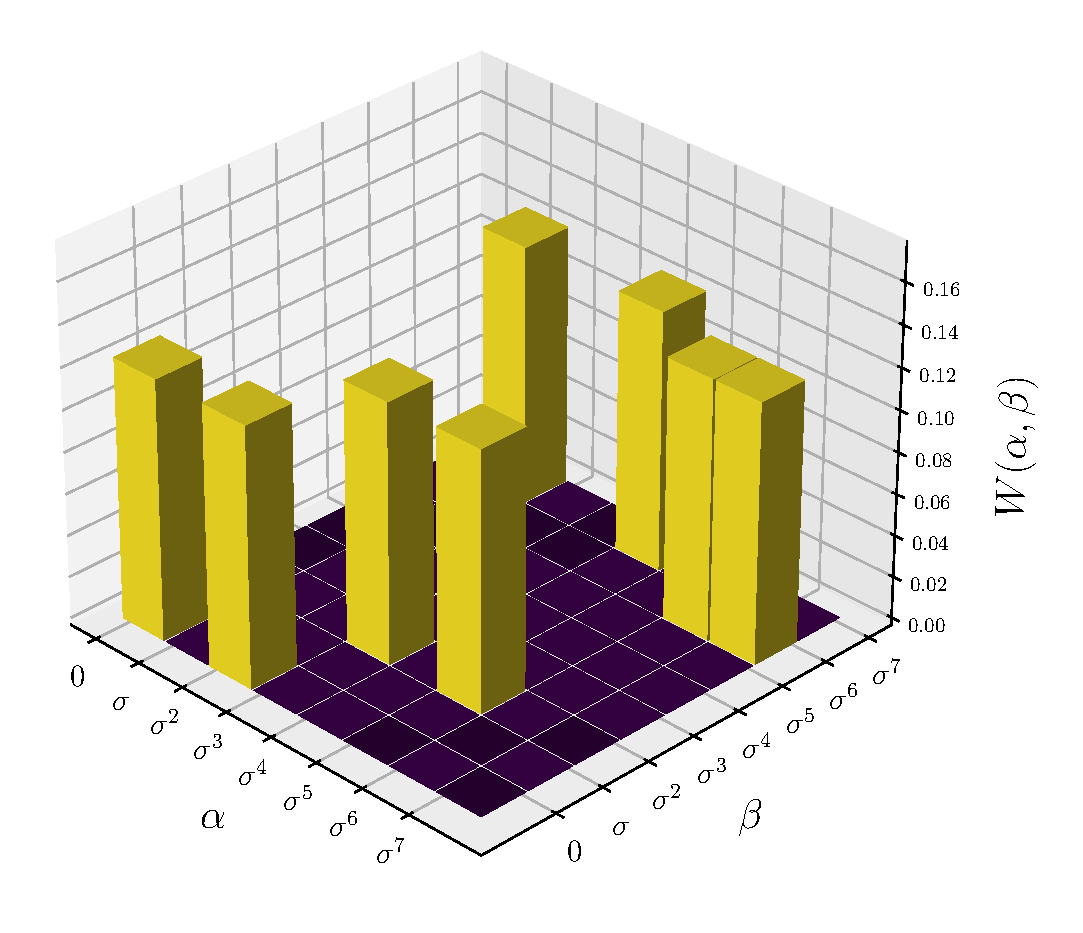
\includegraphics[width=6.5cm]{abelian.eps}
  }}
  \quad 
  \subfloat[\centering Non-abelian curve]{{
    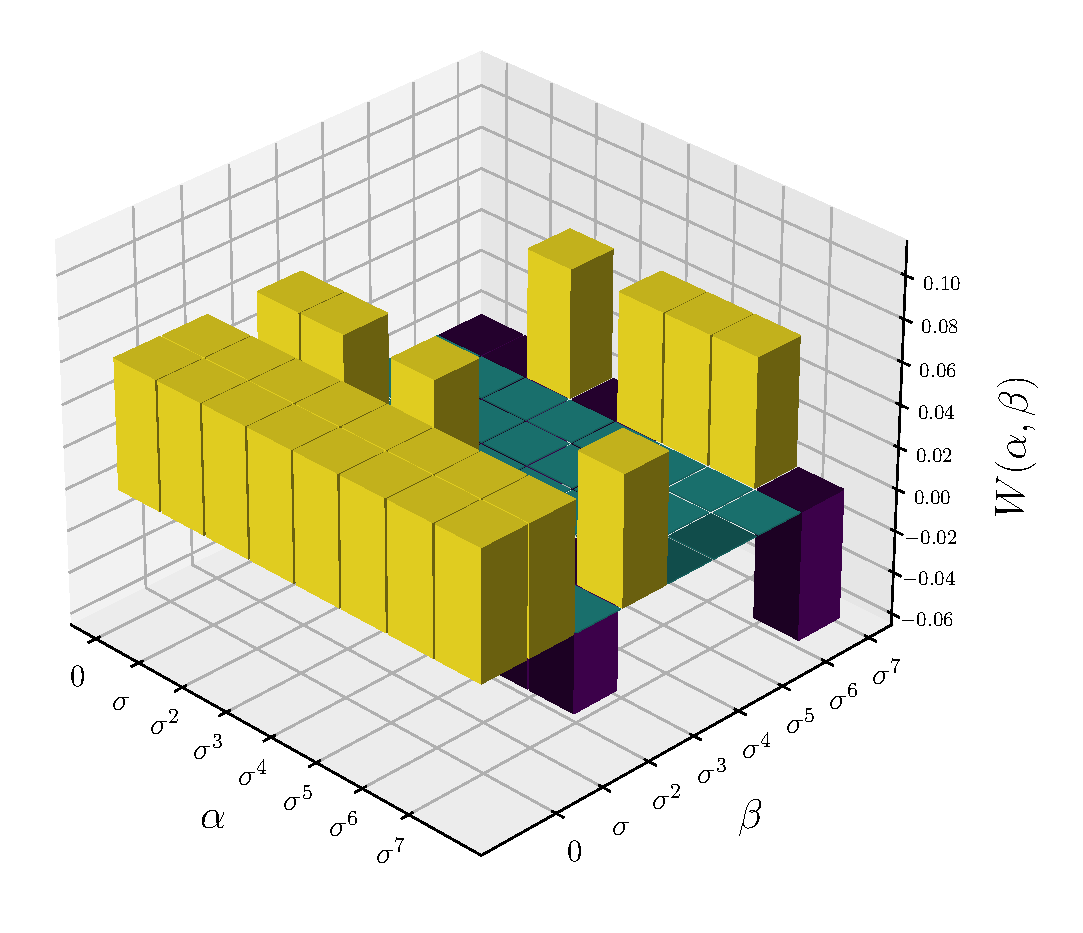
\includegraphics[width=6.5cm]{non_abelian.eps}
  }}
  \caption{
    The Wigner function for the unit stabilizer states corresponding to (a) the
    abelian curve $\protect\beta = \protect\alpha + \protect\sigma^3
    \protect\alpha^2 + \protect\sigma^5 \protect\alpha^4$ (\protect\ref{ac2})
    and (b) the non-abelian curve $\protect\beta = \protect\sigma^2 \protect
    \alpha + \protect\sigma^3 \protect\alpha^2 +
    \protect\sigma^{5}\protect\alpha^{4}$ (\protect\ref{nac}), for the partition
    of the DPS according to Eqs. (\protect\ref{rays}) and (\protect\ref{ray
    dps}). Notice that the first Wigner function has a delta-function form
    (\protect\ref{ac2 delta}) corresponding to the abelian curve, while the
    second function corresponding to a non-abelian curve takes on negative
    values.
  }
  \label{fig2}
\end{figure}

The abovementioned curves \textit{become} abelian for a different assignment of
signs to the phases (\ref{Phib}). For instance, the curve (\ref{nac}) is abelian
by choosing $\Phi_{\alpha,\mu \alpha }(\theta_{k}) = -\sqrt{\chi\left(\mu
\theta_{k}^{2}\right)}$ for any $\mu \neq 0$. Under this assignment, the
following regular curves (\ref{rc}) are abelian:

\begin{enumerate}
  \item if $\phi = \sigma, \sigma^{2}, \sigma^{4}$, then $\phi_{0} = \phi +
    \phi^{2}$;

  \item if $\phi = \sigma^{3}, \sigma^{5}, \sigma^{6}$, then $\phi_{0} = \phi +
    \phi^{2}$;

  \item if $\phi = 1$, $\phi_{0} = 0$.
\end{enumerate}

Additionally, the curve (\ref{nac1}) is abelian under an assignment where the
signs of $\Phi_{\alpha,\mu \alpha}(\theta_{k})$ depend of the value of the slope
$\mu$.

In general, in the three-qubit case and the specific $(3,0,6)$ DPS partition,
certain choices of phase signs $\Phi_{\alpha,\mu \alpha}(\theta_{k})$ can make
all possible commutative curves abelian. The inverse statement is however not
true: for a given curve, it is not always possible to establish a choice of
signs of $\Phi_{\alpha,\beta }(\theta_{k})$ so that this curve becomes abelian
for fixed phases $\Phi_{\alpha,\mu \alpha}(\tau)$.

%%%%%%%%%%%%%%%%%%%%%%%%%%%%%%%%%%%%%%%%%%

\section{Conclusions}

The Wigner mapping kernel can be constructed as a sum of projectors onto
elements of a complete set of MUBs, which are eignestates of disjoint
stabilizers corresponding to a given partition of the discrete phase-space into
non-intersecting commutative curves. Different partitions lead to different
factorization properties of MUBs, which are required for the mapping. For qudit
systems with odd local dimensions, the Wigner kernel is factorized in the same
form for all possible partitions. This results in tomographic universality,
reflected in the delta-function form of Wigner functions of any stabilizer state
corresponding to any partition.

However, in the case of $n$-qubit systems, the mapping kernel is not
factorizable, and its form depends on the chosen discrete phase-space partition
\cite{Bjork2007}, and on the selected set of stabilizer states in this core
partition, particularly on their phases. Consequently, the qubit Discrete Wigner
Function is not tomographically universal for an arbitrary election of phases of
the stabilizer states used for the Wigner map construction. Nonetheless, this
property is not completely lost. It results that for a given partition of the
DPS there are stabilizer states, corresponding to commutative curves which do
not participate in the construction of the mapping kernel, such that their DWF
are delta-functions.  This means that the probability of detecting these states
by measuring in an arbitrary state is obtained by summing the DWF along the
corresponding curve. This property is directly related to the feasibility of
classical simulation of Pauli observables measurements in such $n$-qubit states
(see Theorem 2 in \cite{Raus17}). However, since the measurement procedure is
codified in the partition of the DPS, only some specific stabilizer states,
beyond those used in the measurement scheme, are classically simulable in a
given experimental setup (for a fixed DPS partition). In other words, different
experimental configurations may lead to different classical simulability
outcomes for stabilizer states. This highlights the role of experimental design
and setup in determining the classical or quantum nature of measurement
outcomes. On the other hand, it is always possible to adjust a detection scheme
so that the Pauli measurements in any particular stabilizer state can be
described by a non-contextual hidden variable model.  This supports previously
discussed results \cite{Raus17,contextMagic} that the stabilizer states cannot
be considered as a resource for quantum computation \cite{gottKnill}.

Although we have analyzed only a three-qubit system, the present approach is
extendable to a higher number of qubits. In particular, one can expect that for
any given partition, there are sign assignments such that the DWF of an
arbitrary stabilizer state acquires a delta-function form, i.e. confirms the
tomographic universality of $n$-qubit DWFs under the freedom of the phase
choice. This conjecture has been verified by extensive numerical simulations
and, it can be justified by the same functional form of the recurrence equation
(\ref{phase 2}) for the phase (\ref{Phi}) of any abelian curve.

%%%%%%%%%%%%%%%%%%%%%%%%%%%%%%%%%%%%%%%%%%
\vspace{6pt}

%%%%%%%%%%%%%%%%%%%%%%%%%%%%%%%%%%%%%%%%%%
%% optional
%\supplementary{The following supporting information can be downloaded at:  \linksupplementary{s1}, Figure S1: title; Table S1: title; Video S1: title.}

%%%%%%%%%%%%%%%%%%%%%%%%%%%%%%%%%%%%%%%%%%
\authorcontributions{}

\funding{This research received no external funding.}

\dataavailability{Not applicable.}

\conflictsofinterest{The authors declare no conflict of interest.}

%%%%%%%%%%%%%%%%%%%%%%%%%%%%%%%%%%%%%%%%%
% Optional
\appendixtitles{no} 
% Leave argument "no" if all appendix headings stay EMPTY (then no dot is
% printed after "Appendix A"). If the appendix sections contain a heading then
% change the argument to "yes".
\appendixstart\appendix

\section[\appendixname~\thesection]{}
\label{appA}

\textbf{\color{teal} In this Appendix we derive Eq. (\ref{WF qubit}) of the main
text. Taking into account the expansion inverse to (\ref{Dexp}),}

\begin{equation}
  \color{teal}
  \boldmath
  |\psi_{\kappa }^{\lambda}\rangle \langle \psi_{\kappa }^{\lambda}|
  = \sum_{\tau }\chi (\kappa \tau )\hat{D}^{\lambda }(\tau )
\end{equation}

\textbf{\color{teal} and the representation (\ref{wabD}) of the Wigner kernel,
one obtains}

\begin{adjustwidth}{-\extralength}{0cm}
\begin{equation}
  \color{teal}
  \mathbold
  \langle \psi_{\kappa}^{\lambda}(\pi)
  |\hat{w}\left(\alpha,\beta\,|\,\pi_{0}\right)
  |\psi_{\kappa}^{\lambda}(\pi)\rangle
  = 2^{-n} \sum_{\tau} \sum\limits_{\gamma,\delta}
  \chi\left( \gamma \beta + \delta \alpha \right)\chi(\kappa \tau)
  \Tr\left(
    D\left( \gamma, \delta |\,\pi_{0} \right)
    D\left(
      \alpha_{\lambda}^{\prime}(\tau),\beta_{\lambda}^{\prime }(\tau)|\pi
    \right)
  \right),
\end{equation}
\end{adjustwidth}

\textbf{\color{teal}where the sum over $\tau$ denotes a sum over the points of
  the curve
  $\left(\alpha_{\lambda}^{\prime}(\tau),\beta_{\lambda}^{\prime}(\tau)\right)
  \in \Gamma^{\lambda}(\pi)$; the displacement operators $D\left(\gamma,\delta
  |\,\pi_{0}\right)$ and
  $D\left(\alpha_{\lambda}^{\prime}(\tau),\beta_{\lambda}^{\prime
  }(\tau)|\pi\right)$ from the partitions $\pi_{0}$ and $\pi$ respectively,
  according to (\ref{D}), (\ref{Phi}) carry the corresponding phases
$\Phi_{\gamma,\delta}^{\pi_{0}}$ and
$\Phi_{\alpha^{\prime}(\tau),\beta^{\prime}(\tau )}^{\pi \ast }$, that guarantee
the abelian property (\ref{DD}). Thus, one gets}

\begin{equation}
  \color{teal}
  \boldmath
  \langle \psi_{\kappa}^{\lambda }(\pi)
  |\hat{w}\left(\alpha,\beta\,|\,\pi _{0}\right)
  |\psi_{\kappa}^{\lambda}(\pi)\rangle
  = \sum_{\tau}\sum\limits_{\gamma,\delta}
  \chi\left(\gamma \beta +\delta \alpha\right) \chi (\kappa \tau)
  \Phi_{\gamma,\delta }^{\pi_{0}}
  \Phi_{\alpha^{\prime}(\tau),\beta^{\prime}(\tau)}^{\pi\ast}
  \delta_{\alpha^{\prime }(\tau),\gamma}
  \delta_{\beta^{\prime }(\tau),\delta},
\end{equation}

\textbf{\color{teal}which after performing a sum over $\gamma$ and $\delta$, is
reduced to Eq. (\ref{WF qubit}).}

\section[\appendixname~\thesection]{}
\label{appB}

In this Appendix we recall some basic properties of commutative curves in even
local dimensions. Commuting sets constituted by $2^{n}$ different monomials
(stabilizers)
$\{\hat{Z}_{\alpha_{\lambda}(\tau)}\hat{X}_{\beta_{\lambda}(\tau)}, \, \tau \in
\mathbb{F}_{2^{n}}\}$ are labelled by points of a discrete grid belonging to a
non-singular curve (i.e., with no self-intersection) $\Gamma^{\lambda}$, that
passes through the origin $(\alpha (0),\beta (0))=(0,0)\in \Gamma^{\lambda }$,
and satisfies

\begin{equation*}
  \tr\left( \alpha_{\lambda}(\tau^{\prime})\beta_{\lambda}(\tau) \right)
  = \tr \left( \alpha_{\lambda}(\tau)\beta_{\lambda}(\tau^{\prime }) \right),
  \quad \left( \alpha_{\lambda }(\tau), \beta_{\lambda}(\tau) \right)
  \in \Gamma^{\lambda}.
\end{equation*}

A general parametric form of such a curve is given by

\begin{equation}
  \alpha (\tau)
  = \sum_{k=0}^{n-1}\alpha_{k}\,\tau^{2^{k}}, \qquad \beta(\tau)
  = \sum_{k=0}^{n-1}\beta_{k} \, \tau^{2^{k}},
  \quad \alpha_{k},\beta_{k}\in \mathbb{F}_{2^{n}},
  \label{curve1a}
\end{equation}

where the coefficients $\alpha_k$ and $\beta_k$ are such that $\sum_{m \neq k}
\tr(\alpha_{m}\beta_{k})=0$, which implies

\begin{equation}
  \left[
    \hat{Z}_{\alpha (\tau )}\hat{X}_{\beta (\tau )},
    \hat{Z}_{\alpha(\tau^{\prime })}\hat{X}_{\beta(\tau^{\prime})}
  \right] = 0,
  \qquad \left( \alpha_{\lambda}(\tau),\beta_{\lambda}(\tau) \right)
  \in \Gamma^{\lambda }.
  \label{stab}
\end{equation}

It is worth noting that $n$ appropriately chosen points of the curve, e.g. $\tau
= \{\theta _{1},\ldots,\theta_{n}\}$ are enough to generate the entire curve.
This is because the set of points of these curves form an abelian group where
each element is of order two, and therefore the group is isomorphic to
$\mathbb{Z}_{2}^n$.

The regular curves, which are non-degenerate in at least one of the directions
$\alpha$ or $\beta$ (i.e., they take on all the values of the field in such a
direction), can be represented in the explicit form \cite{GS2},

\begin{equation}
  \beta = f(\alpha)
  = \sum_{k=0}^{n-1} \phi_{k} \, \alpha^{2^{k}}
  \quad \text{or} \quad
  \alpha = g(\beta) = \sum_{k=0}^{n-1} \psi_{k}\,\beta^{2^{k}},
  \label{RC}
\end{equation}

where the coefficients $\phi_{k},\psi_{k} \in \mathbb{F}_{2^{n}}$ satisfy the
following commutativity restrictions,

\begin{equation}
  \phi_{k} = \phi _{n-k}^{2^{k}}\,,
  \qquad \psi_{k} = \psi_{n-k}^{2^{k}}\,,
  \qquad k=1,\ldots, \left\lfloor \frac{n-1}{2}\right\rfloor,
  \label{Acc}
\end{equation}

where $\left\lfloor . \right\rfloor$ denotes the integer part and in particular
for even $n$, the coefficients satisfy the additional restriction: 

\begin{equation}
  \phi_{n/2} = \phi_{n/2}^{2^{n/2}},
  \qquad \psi_{n/2} = \psi_{n/2}^{2^{n/2}}.
\end{equation}

The degenerate (or exceptional) curves are characterized by multiple appearances
of the admissible points in both directions $\alpha $ and $\beta$. In other
words, for every point $(\alpha_{j},\beta_{j})$ of such a curve, $\alpha_{j}$
and $\beta_{j}$ take on only $2^{n-r_{\beta }}$ and $2^{n-r_{\alpha}}$ different
values respectively, where $r_{\alpha }$ and $r_{\beta }$ are the degrees of
degenerations along the corresponding axes.  The admissible points of such
curves are fixed by the relations $\tr(\sigma_{j}\beta)=0$ and
$\tr(\sigma_{k}\alpha)=0$ where $\sigma_{j}, \sigma_{k}$ are some given elements
of $\mathbb{F}_{2^{n}}$.

The partitions of the DPS constituted by $2^{n}+1$ commutative curves are
classified by their factorization structures (\ref{curve_part}), $\lambda =
\{m_{1},m_{2},\ldots ,m_{n}\}\,$, where $\sum_{k}$ $m_{k}=2^{n}+1$, which
indicates the number and the lengths of the commuting sub-blocks of the
stabilizers labelled by the points of a curve. Locally equivalent stabilizers
can be labelled by points of different curves, but have the same factorization
structure. On the other hand, curves with different factorization structures are
not locally equivalent.

In particular, in the partition given by Eq. (\ref{rays}) there are three
completely factorized rays ($\beta = 0, \alpha = 0$, and $\beta = \alpha$),
i.e., of the structure $\{1,1,1\}$, and the other six rays have the structure
$\{3\}$, so that the whole partition is $(3,0,6)$.

The $(0,9,0)$ partitions include only curves with the factorization $\{1,2\}$,
and always contain exceptional curves. One example of these partitions is given
by the following seven regular and two exceptional curves:

\begin{enumerate}
  %\item $\left[label = \alpha*)\right]$

  \item Regular curves 
    \begin{equation}
      \begin{array}{ll}
        \alpha = \sigma^{2}\beta + \sigma^{3}\beta^{2} + \sigma^{5}\beta^{4},
        \qquad\qquad
        & \alpha = \sigma^{6}\beta + \sigma^{3}\beta^{2} + \sigma^{5}\beta^{4},
        \\[5pt] 
        \beta = \sigma^{2}\alpha + \sigma^{3}\alpha^{2} + \sigma^{5}\alpha^{4},
        \qquad\qquad
        & \beta = \sigma^{6}\alpha^{2} + \sigma^{3}\alpha^{4}, \\[5pt] 
        \alpha = \beta + \sigma^{6}\beta^{2} + \sigma^{3}\beta^{4},
        \qquad\qquad
        & \beta = \alpha + \sigma^{3}\alpha^{2} + \sigma^{5}\alpha^{4}, \\[5pt] 
        \alpha = \sigma^{3}\beta^{2} + \sigma^{5}\beta^{4},
        \qquad\qquad
        & 
      \end{array}%
    \end{equation}

  \item Exceptional curves 
    \begin{eqnarray}
      \beta ^{2}+\sigma ^{5}\beta
      &=& \sigma ^{2}\alpha ^{2}+\sigma ^{6}\alpha,
      \qquad \tr(\sigma ^{4}\beta )=0,\quad \tr(\sigma ^{5}\alpha ) = 0;
      \notag \\
      && \\
      \beta^{2}+\sigma ^{2}\beta
      &=& \sigma^{6}\alpha^{2} + \sigma^{5}\alpha,
      \qquad \tr(\sigma^{6}\beta) = 0,
      \quad \tr(\sigma ^{2}\alpha ) = 0.
      \notag
    \end{eqnarray}
\end{enumerate}

\section[\appendixname~\thesection]{}
\label{appC}

\textbf{\color{teal}In this Appendix we provide the explicit expressions for the
  reconstruction of the states $|\psi_{0}^{(\beta;1,\sigma^{5})}(0,9,0)\rangle$
  and $|\psi_{0}^{(\beta ;\sigma^{2},\sigma^{5})}(0,9,0)\rangle$ associated to
  the curves (\ref{ac2}) and (\ref{nac}) in terms of ray-related MUBs projectors
  with the corresponding probabilities (\ref{tom r}):}

\begin{adjustwidth}{-\extralength}{0cm}
\begin{equation}
  \color{teal}
  \boldmath
  |\psi _{0}^{(\beta ;1, \sigma^{5})}(0,9,0)\rangle
  \langle \psi_{0}^{(\beta;1,\sigma^{5})}(0,9,0)|
  = \sum_{\lambda ,\kappa \in \mathbb{F}_{2^{3}}}
  \left( p_{\kappa }^{(\lambda )}(1,\sigma ^{5})-\frac{1}{9}\right)
  |\psi_{\kappa}^{\lambda }\rangle \langle \psi_{\kappa }^{\lambda }|
  + \left( \tilde{p}_{\kappa }(1,\sigma ^{5})-\frac{1}{9}\right)
  |\tilde{\psi}_{\kappa }\rangle \langle \tilde{\psi}_{\kappa }|,
\end{equation}
\end{adjustwidth}

\begin{adjustwidth}{-\extralength}{0cm}
\begin{eqnarray}
  \color{teal}
  \boldmath
  p_{\kappa}^{\lambda}(1,\sigma^{5})
  &=& |\langle \psi_{\kappa }^{\lambda}
  |\psi_{0}^{(\beta ;1,\sigma ^{5})}(0,9,0)\rangle|^{2}
  = \left(\begin{array}{ccccccccc} \lambda \backslash \kappa  & 0 & \sigma  &
      \sigma ^{2} & \sigma ^{3} & \sigma^{4} & \sigma ^{5} & \sigma ^{6} &
      \sigma ^{7} \\ 
    0 & \frac{1}{4} & 0 & \frac{1}{4} & 0 & 0 & 0 & \frac{1}{4} & \frac{1}{4} \\
    [6pt]
    \sigma & \frac{1}{8} & \frac{1}{8} & \frac{1}{8} & \frac{1}{8} & \frac{1}{8}
           & \frac{1}{8} & \frac{1}{8} & \frac{1}{8} \\ [6pt]
    \sigma^{2} & \frac{1}{8} & \frac{1}{8} & \frac{1}{8} & \frac{1}{8} &
    \frac{1}{8} & \frac{1}{8} & \frac{1}{8} & \frac{1}{8} \\  [6pt]
    \sigma^{3} & \frac{1}{4} & 0 & 0 & 0 & \frac{1}{4} & \frac{1}{4} & 0 &
    \frac{1}{4} \\  [6pt] \sigma^{4} & \frac{1}{4} & 0 & 0 & \frac{1}{4} &
    \frac{1}{4} & 0 & \frac{1}{4} & 0 \\  [6pt]
    \sigma^{5} & \frac{1}{8} & \frac{1}{8} & \frac{1}{8} & \frac{1}{8} &
    \frac{1}{8} & \frac{1}{8} & \frac{1}{8} & \frac{1}{8} \\  [6pt] \sigma^{6} &
    \frac{1}{2} & \frac{1}{2} & 0 & 0 & 0 & 0 & 0 & 0 \\  [6pt]
    \sigma^{7} & \frac{1}{4} & 0 & \frac{1}{4} & \frac{1}{4} & 0 & \frac{1}{4} &
    0 & 0
  \end{array}\right), \\
  \tilde{p}_{\kappa }(1,\sigma^{5})
  &=& |\langle \tilde\psi_\kappa | \psi_0^{(\beta;1,\sigma^5)}(0,9,0)\rangle|^2
  = \frac{1}{8},% \quad \text{for all } \kappa \in \mathbb F_{2^3},
\end{eqnarray}
\end{adjustwidth}

\textbf{\color{teal}and}

\begin{adjustwidth}{-\extralength}{0cm}
\begin{equation}
  \color{teal}
  \boldmath
  |\psi_{0}^{(\beta;\sigma^{2},\sigma^{5})}(0,9,0)\rangle
  \langle \psi_{0}^{(\beta ; \sigma^{2},\sigma^{5})}(0,9,0)|
  = \sum_{\lambda }\sum_{\kappa} \left(
    p_{\kappa }^{(\lambda )}\left( \sigma ^{2},\sigma ^{5}\right) -\frac{1}{9}
  \right)
  |\psi_{\kappa}^{\lambda}\rangle \langle \psi_{\kappa}^{\lambda }|
  + \left( \tilde{p}_{\kappa }(\sigma ^{2},\sigma ^{5})-\frac{1}{9} \right)
  |\tilde{\psi}_{\kappa }\rangle \langle \tilde{\psi}_{\kappa }|,
\end{equation}
\end{adjustwidth}

\begin{adjustwidth}{-\extralength}{0cm}
\begin{eqnarray}
  \color{teal}
  \boldmath
  p_{\kappa }^{\lambda }\left(\sigma^{2}, \sigma^{5}\right)
  &=& |\langle\psi_{\kappa }^{\lambda }
  |\psi_{0}^{(\beta ;\sigma ^{2},\sigma^{5})}(0,9,0)\rangle|^{2}
  = \left(\begin{array}{ccccccccc}
    \lambda \backslash \kappa  & 0 & \sigma  & \sigma ^{2} & \sigma ^{3} &
    \sigma ^{4} & \sigma ^{5} & \sigma ^{6} & \sigma ^{7} \\ 
    0 & \frac{1}{2} & \frac{1}{2} & 0 & 0 & 0 & 0 & 0 & 0 \\ [6pt]
    \sigma & \frac{1}{8} & \frac{1}{8} & \frac{1}{8} & \frac{1}{8} &
    \frac{1}{8} & \frac{1}{8} & \frac{1}{8} & \frac{1}{8} \\  [6pt]
    \sigma^{2} & \frac{1}{4} & 0 & \frac{1}{4} & \frac{1}{4} & 0 &
    \frac{1}{4} & 0 & 0 \\  [6pt]
    \sigma^{3} & \frac{1}{4} & 0 & 0 & \frac{1}{4} & \frac{1}{4} & 0 &
    \frac{1}{4} & 0 \\  [6pt]
    \sigma^{4} & 0 & \frac{1}{4} & \frac{1}{4} & \frac{1}{4} & 0 & 0 &
    \frac{1}{4} & 0 \\  [6pt]
    \sigma^{5} & \frac{1}{8} & \frac{1}{8} & \frac{1}{8} & \frac{1}{8} &
    \frac{1}{8} & \frac{1}{8} & \frac{1}{8} & \frac{1}{8} \\  [6pt]
    \sigma^{6} & 0 & \frac{1}{4} & 0 & \frac{1}{4} & \frac{1}{4} &
    \frac{1}{4} & 0 & 0 \\  [6pt]
    \sigma^{7} & \frac{1}{8} & \frac{1}{8} & \frac{1}{8} & \frac{1}{8} &
    \frac{1}{8} & \frac{1}{8} & \frac{1}{8} & \frac{1}{8}
  \end{array}\right), \\
  \tilde{p}_{\kappa }(\sigma^{2},\sigma^{5})
  &=& |\langle \tilde\psi_\kappa | \psi_0^{(\beta;\sigma^2,\sigma^5)}(0,9,0)\rangle|^2
  = \frac{1}{8},% \quad \text{for all } \kappa \in \mathbb F_{2^3},
\end{eqnarray}
\end{adjustwidth}

\textbf{\color{teal}where the MUBs associated with the partition of the DPS in
rays (\ref{rays}) have the form,}

\begin{eqnarray}
  \color{teal}
  \boldmath
  |\psi_{\kappa }^{\lambda }\rangle
  &=& 2^{-3} \sum_{\alpha,\gamma \in \mathbb{F}_{2^{3}}}
  \Phi_{\alpha,\lambda \alpha} \;
  %(-1)^{\tr(\alpha (\kappa + \gamma))}
  \chi\left( \alpha(\kappa+\gamma) \right) 
  |\gamma \rangle, \\ [6pt]
  |\tilde{\psi}_{\kappa }\rangle
  &=& 2^{-3 / 2} \sum_{\gamma \in \mathbb{F}_{2^{3}}}
  %(-1)^{\tr(\kappa \gamma)}
  \chi\left( \kappa\gamma \right) 
  |\gamma \rangle,
\end{eqnarray}

\textbf{\color{teal}and the phases $\Phi_{\alpha,\beta}$ are defined in
(\ref{ray dps}).}

%%%%%%%%%%%%%%%%%%%%%%%%%%%%%%%%%%%%%%%%%%
\begin{adjustwidth}{-\extralength}{0cm}
%\printendnotes[custom] % Un-comment to print a list of endnotes

\reftitle{References}

% Please provide either the correct journal abbreviation (e.g. according to the
% "List of Title Word Abbreviations" http://www.issn.org/services/online-services/access-to-the-ltwa/) or the full name of the journal.
% Citations and References in Supplementary files are permitted provided that they also appear in the reference list here. 

%=====================================
% References, variant A: external bibliography
%=====================================
%\bibliography{your_external_BibTeX_file}

%=====================================
% References, variant B: internal bibliography
%=====================================
\begin{thebibliography}{999}
% Reference 1
\bibitem{wigner} Wigner, E. On the quantum correction for thermodynamic
equilibrium. \textit{Phys. Rev. A} \textbf{1932}, \textit{40}, 749-759,
doi:10.1103/PhysRev.40.749.
% Reference 2
\bibitem{bloch} Bloch, F. Zur Theorie des Austauschproblems und der
Remanenzerscheinung der Ferromagnetika. \textit{Zeits F. Physik} \textbf{1932},
\textit{74}, 295-335, doi:10.1007/978-3-662-41138-4.
% Reference 3
\bibitem{groenewold} Groenewold, H. J. On the principles of elementary
quantum mechanics. \textit{Physica} \textbf{1949}, \textit{12}, 405-460,
doi:10.1016/S0031-8914(46)80059-4.
% Reference 4
\bibitem{moyal} Moyal, J. E. Quantum mechanics as a statistical theory. 
\textit{Mathematical Proceedings of the Cambridge Philosophical Society} 
\textbf{1947}, \textit{45}, 99-124, doi:10.1017/S0305004100000487.
% Reference 5
\bibitem{qoptics} Mandel, L.; Wolf, E. Coherence Properties of Optical
Fields. \textit{Rev. Mod. Phys.} \textbf{1965}, \textit{37}, 231-287,
doi:10.1103/RevModPhys.37.231.
% Reference 6
\bibitem{electron1} Barker, J. R.; Murray, S. A quasi-classical formulation
of the Wigner function approach to quantum ballistic transport. \textit{Phys.
Lett. A} \textbf{1983}, \textit{93}, 271-274, doi:10.1016/0375-9601(83)90786-7.
% Reference 7
\bibitem{electron2} Lin, J.; Chiu, L. C. Quantum theory of electron
transport in the Wigner formalism. \textit{J. Appl. Phys.} \textbf{1985}, 
\textit{57}, 1373-1376, doi:10.1063/1.334489.
% Reference 8
\bibitem{berry} Berry, M. V. Semi-classical mechanics in phase space: A
study of Wigner's function. \textit{Philos. Trans. R. Soc. A} \textbf{1977}, 
\textit{287}, 237-271, doi:10.1098/rsta.1977.0145.
% Reference 9
\bibitem{spin1} O'Connell R. F.; Wigner E. P. Manifestations of Bose and
Fermi statistics on the quantum distribution functionfor systems of spin-0
and spin- 1/2 particles. \textit{Phys. Rev. A} \ textbf{1984}, \textit{30},
2613-2618, doi:10.1103/PhysRevA.30.2613.
% Reference 10
\bibitem{spin2} Cohen, M.; Scully, M. O. Joint Wigner distribution for
spin-1/2 particles. \textit{Foud. Phys.} \textbf{1986}, \textit{16},
295-310., doi:10.1007/BF01882690.
% Reference 11
\bibitem{wootters1} Wootters, W. K. A Wigner-function formulation of
finite-state quantum mechanics. \textit{Annals Phys.} \textbf{1987},
\textit{176}, 1-21, doi:10.1016/0003-4916(87)90176-X.
% Reference 12
\bibitem{gibbons} Gibbons, K. S.; Hoffman, M. J.; Wootters, W. K. Discrete
phase space based on finite fields. \textit{Phys. Rev. A} \textbf{2004}, 
\textit{70}, 062101, doi:10.1103/PhysRevA.70.062101.
% Reference 13
\bibitem{gottKnill} Gottesman, D. The Heisenberg representation of quantum
computers. In \textit{Group 22: International Colloquium on Group
Theoretical Methods in Physics}, Proceedings of 22nd International
Colloquium, Group22, ICGTMP'98, Hobart, Australia, July 13-17, 1998; S. P.
Corney, R. Delbourgo, P. D. Jarvis, Eds.; International Press: Cambridge,
MA, 1999, pp. 32-43.
% Reference 14
\bibitem{galvao} Galv\~ao, E.F. Discrete Wigner functions and quantum
computational speedup. \textit{Phys. Rev. A} \textbf{2005}, \textit{71},
042302, doi:10.1103/PhysRevA.71.042302.
% Reference 15
\bibitem{cormick} Cormick, C.; \textit{et al.} Classicality in discrete
Wigner functions. \textit{Phys. Rev. A} \textbf{2006}, \textit{73}, 012301,
doi:10.1103/PhysRevA.73.012301.
% Reference 16
\bibitem{gross} Gross, D. Hudson's theorem for
finite-dimensional quantum systems. \textit{J. Math. Phys. A} \textbf{2006}, 
\textit{47}, 122107, doi:10.1063/1.2393152.
% Reference 17
\bibitem{WignerNegResource} Veitch, V. C.; Ferrie, C.; Gross, D.; Emerson,
J. Negative quasi-probability as a resource for quantum computation. \textit{New
J. Phys.} \textbf{2012}, \textit{14}, 113011,
doi:10.1088/1367-2630/14/11/113011.
% Reference 18
\bibitem{Raus17} Raussendorf, R.; Browne, D.E.; Delfosse, N.; Okay, C.;
Bermejo-Vega, J. Contextuality and Wigner-function negativity in qubit
quantum computation. \textit{Phys. Rev. A} \textbf{2017}, \textit{95}
052334, doi:10.1103/PhysRevA.95.052334.
% Reference 19
\bibitem{UniqueWF} Schmid, D.; Du, H.; Shelby, J. H.; Pusey, M. F.
Uniqueness of Noncontextual Models for Stabilizer Subtheories. \textit{Phys.
Rev. Lett.} \textbf{2022}, \textit{129}, 120403,
doi:10.1103/PhysRevLett.129.120403.
% Reference 20
\bibitem{cohomo} Raussendorf, R.; Okay, C.; Zurel, M.; Feldmann, P. The role
of cohomology in quantum computation with magic states. \textit{Quantum} 
\textbf{2023}, \textit{7}, 979, doi:10.22331/q-2023-04-13-979.
% Reference 21
\bibitem{Saniga2004} Saniga, M.;Planat, M.; Rosu, H. Mutually unbiased bases
and finite projective planes. \textit{\ J. Opt. B: Quantum Semiclass. Opt.} 
\textbf{2004}, \textit{6} L19-L20, doi:10.1088/1464-4266/6/9/L01.
% Reference 22
\bibitem{ivanovic} Ivanovic, I. D. Geometrical description of quantal state
determination. \textit{J. Phys. A.} \textbf{1984}, \textbf{14}, 3241-3245,
doi:10.1088/0305-4470/14/12/019.
% Reference 23
\bibitem{mubs1} Wootters, W. K.; Fields, B. D. Optimal State-Determination
by Mutually Unbiased Measurements. \textit{Ann. Phys.} \textbf{1989}, 
\textit{191} 363-381, doi:10.1016/0003-4916(89)90322-9.
% Reference 24
\bibitem{mubs2} Klappenecker, A.; R{\"{o}}tteler, M. Constructions of
mutually unbiased bases. In \textit{Lecture Notes in Computer Science Vol.
2948: Finite Fields and Applications}, Procceedings of 7th International
Conference, Fq7, Toulouse, France, May 5-9, 2003; G.~Mullen, A.~Poli,
H.~Stichtenoth, Eds. Springer: Germany, Berlin, 2003, pp. 137--144.
% Reference 25
\bibitem{Bandyopadhyay2002} Bandyopadhyay, S.; Boykin, P.~O.;Roychowdhury,
V.; Vatan, F. A new proof for the existence of mutually unbiased bases. 
\textit{Algorithmica} \textbf{2002}, \textit{34}, 512--528,
doi:10.1007/s00453-002-0980-7.
% Reference 26
\bibitem{GS2} Klimov, A. B.; Romero, J. L.; Bj\"{o}rk, G.; S\'{a}nchez-Soto,
L. L. Discrete phase-space structure of n-qubit mutually unbiased bases. 
\textit{Ann.Phys.} \textbf{2009}, \textit{324}, 53-72,
doi:10.1016/j.aop.2008.10.003.
% Reference 27
\bibitem{JPA09} Klimov, A. B.; Romero, J. L.; Bj{\"{o}}rk, G.; S{\'{a}}%
nchez-Soto, L. L. Geometrical approach to mutually unbiased bases. \textit{%
J. Phys. A: Math. Gen.} \textbf{2007}, \textit{40}, 9177,
doi:10.1088/1751-8113/40/14/014.
% Reference 28
\bibitem{Bjork2007} Pittenger, A.~O.; Rubin, M.~H. Wigner functions and
separability for finite systems. \textit{J. Phys. A: Math. Gen.} \textbf{2005%
}, \textit{38} 6005-6036, doi:10.1088/0305-4470/38/26/012.
% Reference 29
\bibitem{DFW11} Wootters, W.K.; A Wigner-function formulation of
finite-state quantum mechanics. \textit{Ann. Phys.} \textbf{1987}, \textit{\
176}, 1-21, doi:10.1016/0003-4916(87)90176-X.
% Reference 30
\bibitem{DFW12} Delfosse, N.; Guerin, P.A.; Bian, J.; Raussendorf, R. Wigner
Function Negativity and Contextuality in Quantum Computation on Rebits. 
\textit{Phys.Rev. X} \textbf{\ 2105 }, \textit{5}, 021003,
doi:10.1016/0003-4916(87)90176-X.
% Reference 31
\bibitem{contextMagic} Howard, M.; Wallman, J.; Vietch, V.; Emerson, J.
Contextuality supplies the `magic' for quantum computation. \textit{Nature}
\textbf{214}, \textit{510}, 351-355, doi:10.1038/nature13460.
% Reference 32
\bibitem{WignerContext} Delfosse, N. \textit{et al.} Equivalence between
contextuality and negativity of the Wigner function for qudits. \textit{New
J. Phys.} \textbf{2017}, \textit{19}, 123024, doi:10.1088/1367-2630/aa8fe3.
% Reference 33
\bibitem{qip17} Mu\~noz, C.; Klimov, A. B.; Sanchez-Soto, L. L. Discrete
phase-space structures and Wigner functions for $N$ qubits. \textit{Quantum
Inf. Process} \textbf{2017}, \textit{16}, 158, doi:10.1007/s11128-017-1607-x.
% Reference 34
\bibitem{FF} Lidl, R.; Niederreiter, H. \textit{Introduction to Finite
Fields and their Applications}, 2nd ed.; Cambridge University Press,
Cambridge, United Kingdom, 1994, ISBN 978-052-146-094-1.
% Reference 35
\bibitem{Schwinger1} Schwinger, J. UNITARY OPERATOR BASES. \textit{Proc.
Natl. Acad. Sci. USA} \textbf{1960}, \textit{46}, 570,
doi:10.1073/pnas.46.4.570.
% Reference 36
\bibitem{Schwinger2} Schwinger, J. UNITARY TRANSFORMATIONS AND THE ACTION
PRINCIPLE. \textit{Proc. Natl. Acad. Sci. USA} \textbf{1960}, \textit{46},
883, doi:10.1073/pnas.46.6.883.
% Reference 37
\bibitem{factor1} Lawrence, J.; Brukner, \v{C}.; Zeilinger, A. Mutually
unbiased binary observable sets on $N$ qubits. \textit{Phys. Rev. A} \textbf{%
2002}, \textit{65}, 032320, doi:10.1103/PhysRevA.65.032320.
% Reference 38
\bibitem{factor2} Romero, J. L.; Bj\"{o}rk, G.; Klimov, A. B.; S\'{a}%
nchez-Soto, L. L. Structure of the sets of mutually unbiased bases for $N$
qubits. \textit{Phys. Rev. A} \textbf{2005}, \textit{72}, 062310,
doi:10.1103/PhysRevA.72.062310.
% Reference 39
\bibitem{Durt2006} Durt, T. About Weyl and Wigner tomography in
finite-dimensional Hilbert spaces. \textit{Open Sys. Inf. Dyn.} \textbf{2006}%
, \textit{13}, 403--413, doi:10.1007/s11080-006-9022-2.
% Reference 40
\bibitem{DFW2-1} Vourdas, A. Quantum systems with finite Hilbert space. 
\textit{Rep. Prog. Phys.} \textbf{2004}, \textit{67}, 267,
doi:10.1088/0034-4885/67/3/R03.
% Reference 41
\bibitem{DFW2-2} Vourdas, A. Factorization in finite quantum systems. 
\textit{\ J. Phys. A: Math. Gen.} \textbf{2003}, \textit{36}, 5645,
doi:10.1088/0305-4470/36/20/319.
% Reference 42
\bibitem{DFW2-3} Paz, J.P.; Roncaglia, A. J.; Saraceno, M. Qubits in phase
space: Wigner-function approach to quantum-error correction and the
mean-king problem. \textit{\ Phys. Rev. A} \textbf{2005}, \textit{72},
012309, doi:10.1103/PhysRevA.72.012309.
% Reference 43
\bibitem{DFW2-4} Bjork, G.; Klimov, A. B.; Sanchez-Soto, L.L. The discrete
Wigner function. In \textit{Progress in Optics}, 1st ed.; Wolf, E., Ed.;
Elsevier: Amsterdam, The Netherlands, 2008, Volume 51, pp. 469-516,
doi:10.1016/S0079-6638(07)51007-3.
% Reference 44
\bibitem{klimov06} Klimov, A. B.; Mu\~{n}oz, C.; Romero, J. L. Geometrical
approach to the discrete Wigner function in prime power dimensions. \textit{%
J. Phys. A: Math. Gen.} \textbf{2006}, \textit{39}, 14471,
doi:10.1088/0305-4470/39/46/016.
\end{thebibliography}

% If authors have biography, please use the format below
%\section*{Short Biography of Authors}
%\bio
%{\raisebox{-0.35cm}{\includegraphics[width=3.5cm,height=5.3cm,clip,keepaspectratio]{Definitions/author1.pdf}}}
%{\textbf{Firstname Lastname} Biography of first author}
%
%\bio
%{\raisebox{-0.35cm}{\includegraphics[width=3.5cm,height=5.3cm,clip,keepaspectratio]{Definitions/author2.jpg}}}
%{\textbf{Firstname Lastname} Biography of second author}

% For the MDPI journals use author-date citation, please follow the formatting guidelines on http://www.mdpi.com/authors/references
% To cite two works by the same author: \citeauthor{ref-journal-1a} (\citeyear{ref-journal-1a}, \citeyear{ref-journal-1b}). This produces: Whittaker (1967, 1975)
% To cite two works by the same author with specific pages: \citeauthor{ref-journal-3a} (\citeyear{ref-journal-3a}, p. 328; \citeyear{ref-journal-3b}, p.475). This produces: Wong (1999, p. 328; 2000, p. 475)

%%%%%%%%%%%%%%%%%%%%%%%%%%%%%%%%%%%%%%%%%%
%% for journal Sci
%\reviewreports{\\
%Reviewer 1 comments and authors' response\\
%Reviewer 2 comments and authors' response\\
%Reviewer 3 comments and authors' response
%}
%%%%%%%%%%%%%%%%%%%%%%%%%%%%%%%%%%%%%%%%%%
\PublishersNote{}
\end{adjustwidth}
\end{document}
